% Options for packages loaded elsewhere
\PassOptionsToPackage{unicode}{hyperref}
\PassOptionsToPackage{hyphens}{url}
\PassOptionsToPackage{dvipsnames,svgnames,x11names}{xcolor}
%
\documentclass[
  12pt,
  oneside]{book}
\usepackage{amsmath,amssymb}
\usepackage{lmodern}
\usepackage{iftex}
\ifPDFTeX
  \usepackage[T1]{fontenc}
  \usepackage[utf8]{inputenc}
  \usepackage{textcomp} % provide euro and other symbols
\else % if luatex or xetex
  \usepackage{unicode-math}
  \defaultfontfeatures{Scale=MatchLowercase}
  \defaultfontfeatures[\rmfamily]{Ligatures=TeX,Scale=1}
\fi
% Use upquote if available, for straight quotes in verbatim environments
\IfFileExists{upquote.sty}{\usepackage{upquote}}{}
\IfFileExists{microtype.sty}{% use microtype if available
  \usepackage[]{microtype}
  \UseMicrotypeSet[protrusion]{basicmath} % disable protrusion for tt fonts
}{}
\makeatletter
\@ifundefined{KOMAClassName}{% if non-KOMA class
  \IfFileExists{parskip.sty}{%
    \usepackage{parskip}
  }{% else
    \setlength{\parindent}{0pt}
    \setlength{\parskip}{6pt plus 2pt minus 1pt}}
}{% if KOMA class
  \KOMAoptions{parskip=half}}
\makeatother
\usepackage{xcolor}
\usepackage{color}
\usepackage{fancyvrb}
\newcommand{\VerbBar}{|}
\newcommand{\VERB}{\Verb[commandchars=\\\{\}]}
\DefineVerbatimEnvironment{Highlighting}{Verbatim}{commandchars=\\\{\}}
% Add ',fontsize=\small' for more characters per line
\usepackage{framed}
\definecolor{shadecolor}{RGB}{248,248,248}
\newenvironment{Shaded}{\begin{snugshade}}{\end{snugshade}}
\newcommand{\AlertTok}[1]{\textcolor[rgb]{0.94,0.16,0.16}{#1}}
\newcommand{\AnnotationTok}[1]{\textcolor[rgb]{0.56,0.35,0.01}{\textbf{\textit{#1}}}}
\newcommand{\AttributeTok}[1]{\textcolor[rgb]{0.77,0.63,0.00}{#1}}
\newcommand{\BaseNTok}[1]{\textcolor[rgb]{0.00,0.00,0.81}{#1}}
\newcommand{\BuiltInTok}[1]{#1}
\newcommand{\CharTok}[1]{\textcolor[rgb]{0.31,0.60,0.02}{#1}}
\newcommand{\CommentTok}[1]{\textcolor[rgb]{0.56,0.35,0.01}{\textit{#1}}}
\newcommand{\CommentVarTok}[1]{\textcolor[rgb]{0.56,0.35,0.01}{\textbf{\textit{#1}}}}
\newcommand{\ConstantTok}[1]{\textcolor[rgb]{0.00,0.00,0.00}{#1}}
\newcommand{\ControlFlowTok}[1]{\textcolor[rgb]{0.13,0.29,0.53}{\textbf{#1}}}
\newcommand{\DataTypeTok}[1]{\textcolor[rgb]{0.13,0.29,0.53}{#1}}
\newcommand{\DecValTok}[1]{\textcolor[rgb]{0.00,0.00,0.81}{#1}}
\newcommand{\DocumentationTok}[1]{\textcolor[rgb]{0.56,0.35,0.01}{\textbf{\textit{#1}}}}
\newcommand{\ErrorTok}[1]{\textcolor[rgb]{0.64,0.00,0.00}{\textbf{#1}}}
\newcommand{\ExtensionTok}[1]{#1}
\newcommand{\FloatTok}[1]{\textcolor[rgb]{0.00,0.00,0.81}{#1}}
\newcommand{\FunctionTok}[1]{\textcolor[rgb]{0.00,0.00,0.00}{#1}}
\newcommand{\ImportTok}[1]{#1}
\newcommand{\InformationTok}[1]{\textcolor[rgb]{0.56,0.35,0.01}{\textbf{\textit{#1}}}}
\newcommand{\KeywordTok}[1]{\textcolor[rgb]{0.13,0.29,0.53}{\textbf{#1}}}
\newcommand{\NormalTok}[1]{#1}
\newcommand{\OperatorTok}[1]{\textcolor[rgb]{0.81,0.36,0.00}{\textbf{#1}}}
\newcommand{\OtherTok}[1]{\textcolor[rgb]{0.56,0.35,0.01}{#1}}
\newcommand{\PreprocessorTok}[1]{\textcolor[rgb]{0.56,0.35,0.01}{\textit{#1}}}
\newcommand{\RegionMarkerTok}[1]{#1}
\newcommand{\SpecialCharTok}[1]{\textcolor[rgb]{0.00,0.00,0.00}{#1}}
\newcommand{\SpecialStringTok}[1]{\textcolor[rgb]{0.31,0.60,0.02}{#1}}
\newcommand{\StringTok}[1]{\textcolor[rgb]{0.31,0.60,0.02}{#1}}
\newcommand{\VariableTok}[1]{\textcolor[rgb]{0.00,0.00,0.00}{#1}}
\newcommand{\VerbatimStringTok}[1]{\textcolor[rgb]{0.31,0.60,0.02}{#1}}
\newcommand{\WarningTok}[1]{\textcolor[rgb]{0.56,0.35,0.01}{\textbf{\textit{#1}}}}
\usepackage{longtable,booktabs,array}
\usepackage{calc} % for calculating minipage widths
% Correct order of tables after \paragraph or \subparagraph
\usepackage{etoolbox}
\makeatletter
\patchcmd\longtable{\par}{\if@noskipsec\mbox{}\fi\par}{}{}
\makeatother
% Allow footnotes in longtable head/foot
\IfFileExists{footnotehyper.sty}{\usepackage{footnotehyper}}{\usepackage{footnote}}
\makesavenoteenv{longtable}
\usepackage{graphicx}
\makeatletter
\def\maxwidth{\ifdim\Gin@nat@width>\linewidth\linewidth\else\Gin@nat@width\fi}
\def\maxheight{\ifdim\Gin@nat@height>\textheight\textheight\else\Gin@nat@height\fi}
\makeatother
% Scale images if necessary, so that they will not overflow the page
% margins by default, and it is still possible to overwrite the defaults
% using explicit options in \includegraphics[width, height, ...]{}
\setkeys{Gin}{width=\maxwidth,height=\maxheight,keepaspectratio}
% Set default figure placement to htbp
\makeatletter
\def\fps@figure{htbp}
\makeatother
\setlength{\emergencystretch}{3em} % prevent overfull lines
\providecommand{\tightlist}{%
  \setlength{\itemsep}{0pt}\setlength{\parskip}{0pt}}
\setcounter{secnumdepth}{5}
\usepackage{booktabs,multirow,color,eurosym}
\usepackage{amsthm}
\usepackage{multicol}
\usepackage{geometry}
\usepackage[natbibapa]{apacite}
\usepackage{txfonts} %txfonts iwona lmodern
\usepackage{hyperref}

\renewcommand{\texteuro}{\text{\euro}} 
%\hypersetup{colorlinks=false, pdfborderstyle={/S/U/W 1} }

%\geometry{executivepaper}
\geometry{a4paper}
\usepackage{makeidx}
%\usepackage{imakeidx} % Uncomment to get correct page numbers in index
\makeindex




%% Note: Pandoc (which is doing all of the output conversion behind the scenes) does not parse the content of LaTeX environments. This creates problems when you try to include LaTeX commands with curly brackets directly in your Rmd file. E.g. You can't just use `\begin{multicols}{2}` directly in your Rmd file. Luckily, a straightforward workaround is to simply define some new shortcut commands yourself as per the below.
%% See: https://stackoverflow.com/questions/25849814/rstudio-rmarkdown-both-portrait-and-landscape-layout-in-a-single-pdf/27334272#27334272
\newcommand{\btwocol}{\begin{multicols}{2}}
\newcommand{\etwocol}{\end{multicols}}


\usepackage{tikz}
\ifLuaTeX
  \usepackage{selnolig}  % disable illegal ligatures
\fi
\usepackage[]{natbib}
\bibliographystyle{apacite}
\IfFileExists{bookmark.sty}{\usepackage{bookmark}}{\usepackage{hyperref}}
\IfFileExists{xurl.sty}{\usepackage{xurl}}{} % add URL line breaks if available
\urlstyle{same} % disable monospaced font for URLs
\hypersetup{
  pdftitle={How to Use R for Data Science},
  pdfauthor={© Prof.~Dr.~Stephan Huber (Stephan.Huber@hs-fresenius.de)},
  colorlinks=true,
  linkcolor={red},
  filecolor={Maroon},
  citecolor={Blue},
  urlcolor={blue},
  pdfcreator={LaTeX via pandoc}}

\title{How to Use R for Data Science}
\usepackage{etoolbox}
\makeatletter
\providecommand{\subtitle}[1]{% add subtitle to \maketitle
  \apptocmd{\@title}{\par {\large #1 \par}}{}{}
}
\makeatother
\subtitle{Lecture Notes}
\author{© Prof.~Dr.~Stephan Huber (\href{mailto:Stephan.Huber@hs-fresenius.de}{\nolinkurl{Stephan.Huber@hs-fresenius.de}})}
\date{Last compiled on 26 April, 2023}

\usepackage{amsthm}
\newtheorem{theorem}{Theorem}[chapter]
\newtheorem{lemma}{Lemma}[chapter]
\newtheorem{corollary}{Corollary}[chapter]
\newtheorem{proposition}{Proposition}[chapter]
\newtheorem{conjecture}{Conjecture}[chapter]
\theoremstyle{definition}
\newtheorem{definition}{Definition}[chapter]
\theoremstyle{definition}
\newtheorem{example}{Example}[chapter]
\theoremstyle{definition}
\newtheorem{exercise}{Exercise}[chapter]
\theoremstyle{definition}
\newtheorem{hypothesis}{Hypothesis}[chapter]
\theoremstyle{remark}
\newtheorem*{remark}{Remark}
\newtheorem*{solution}{Solution}
\begin{document}
\maketitle

{
\hypersetup{linkcolor=}
\setcounter{tocdepth}{2}
\tableofcontents
}
\hypertarget{preface}{%
\chapter*{Preface}\label{preface}}
\addcontentsline{toc}{chapter}{Preface}

\hypertarget{about-the-notes}{%
\section*{About the notes}\label{about-the-notes}}

\begin{itemize}
\tightlist
\item
  This script aims to support my lecture at the HS Fresenius. It is incomplete and no substitute for taking actively part in class.
\item
  The old version of the notes can be found here PDF.
\item
  I appreciate you reading it, and I appreciate any comments.
\item
  This is work in progress so please check for updates regularly.
\item
  The lecture notes are available online or you can download it as a \href{https://raw.githubusercontent.com/hubchev/hubchev.github.io/main/ds/_main.pdf}{pdf file here}
\item
  These notes are published under a Creative Commons BY-SA license (CC BY-SA) version 4.0. This means it can be reused, remixed, retained, revised and redistributed as long as appropriate credit is given to the authors. If you remix, or modify the original version of this open textbook, you must redistribute all versions of this open textbook under the same license---CC BY-SA. This script is build on the work of \citet{Navarro2020Learning}, \citet{Muschelli2022Introduction}, \citet{Thulin2021Modern}, and \citet{Ismay2022Statistical} which is also published under CC BY-SA.
\end{itemize}

\hypertarget{about-the-author}{%
\section*{About the author}\label{about-the-author}}

\begin{figure}
\centering
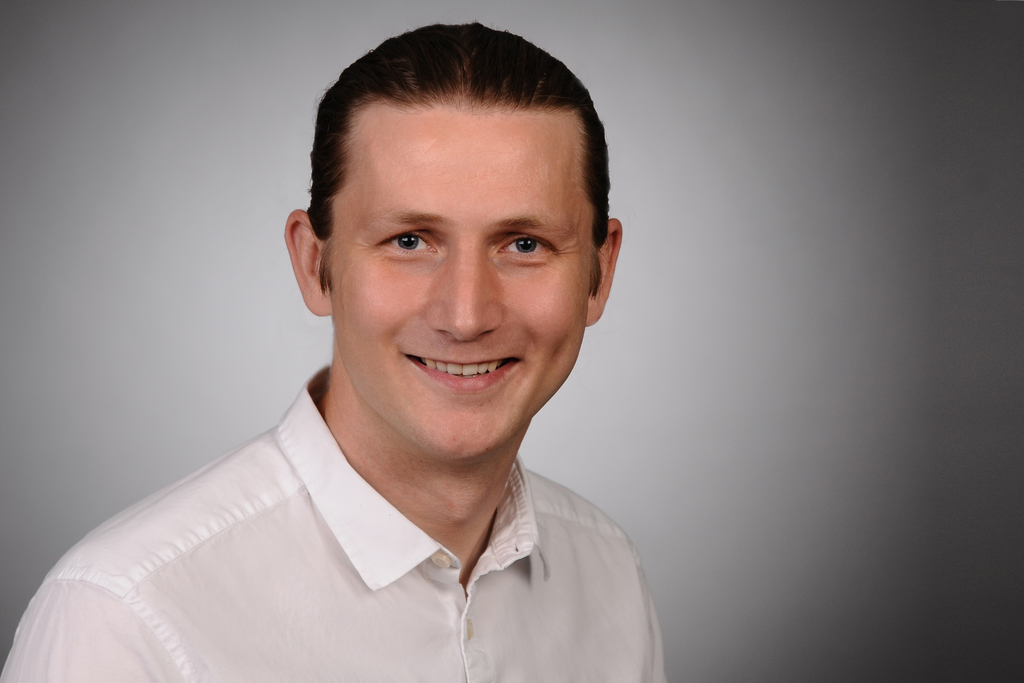
\includegraphics[width=0.25\textwidth,height=\textheight]{fig/huber2.jpeg}
\caption[\label{fig:itsme} Prof.~Dr.~Stephan Huber]{\label{fig:itsme} Prof.~Dr.~Stephan Huber\footnotemark{}}
\end{figure}
\footnotetext{Picture is taken from \url{https://sites.google.com/view/stephanhuber}}

Prof.~Dr.~Stephan Huber is Professor of International Economics and Data Science at \emph{HS Fresenius} and holds a Diploma in Economics from the \emph{University of Regensburg} and a Doctoral Degree (summa cum laude) from the University of Trier. He completed postgraduate studies at the \emph{Interdisciplinary Graduate Center of Excellence at the Institute for Labor Law and Industrial Relations in the European Union (IAAEU)} in Trier. He was a research assistant to Prof.~Dr.~Dr.~h.c. Joachim Möller at the \emph{University of Regensburg}, post-doc at the \emph{Leibniz Institute for East and Southeast European Studies (IOS)} in Regensburg and freelancer at \emph{Charles University} in Prague.

He has worked as a lecturer at various institutions including the \emph{TU Munich}, the \emph{University of Regensburg}, \emph{Saarland University}, and the \emph{Universities of Applied Sciences in Frankfurt and Augsburg}. He has also taught abroad for the \emph{University of Cordoba} in Spain and the \emph{University of Perugia}. Professor Huber has published his work in international journals such as the \emph{Canadian Journal of Economics} and the \emph{Stata Journal}. More on his work can be found on his private homepage \href{https://www.t1p.de/stephanhuber}{www.t1p.de/stephanhuber}.

\textbf{Contact}

\begin{verbatim}
   Hochschule Fresenius für Wirtschaft & Medien GmbH
   Im MediaPark 4c
   50670 Cologne
   
   Office: 4b OG-1 Bü01 (Office hour: Thursday 1-2 p.m.)
   Telefon: +49 221 973199-523
   Mail: stephan.huber@hs-fresenius.de
   Private homepage: www.t1p.de/stephanhuber
   Github: https://github.com/hubchev
\end{verbatim}

\hypertarget{getting-started}{%
\chapter{Getting Started with R}\label{getting-started}}

Before we can start exploring data in R, there are some key concepts to understand first:

\begin{enumerate}
\def\labelenumi{\arabic{enumi}.}
\tightlist
\item
  Why R?
\item
  How to learn R?
\item
  What are R and RStudio?
\item
  How to use R and RStudio without installation
\item
  How to install R and RStudio
\item
  How to write and run code in R
\item
  What are R packages?
\end{enumerate}

\hypertarget{sec:whyR}{%
\section{Why R?}\label{sec:whyR}}

R is a free and open-source programming language that provides a wide range of advanced statistics capabilities, state-of-the-art graphics, and powerful data manipulation capabilities. It supports larger data sets, reads any type of data, and runs on multiple platforms. R makes it easier to automate tasks, organize projects, ensure reproducibility, and find and fix errors, and anyone can contribute packages to improve its functionality. Moreover, the following points are worth to emphasize:

\begin{itemize}
\tightlist
\item
  \textbf{R is an artist!} Check out:

  \begin{itemize}
  \tightlist
  \item
    \url{https://www.r-graph-gallery.com/}
  \item
    \url{http://r-statistics.co/Top50-Ggplot2-Visualizations-MasterList-R-Code.html}
  \item
    \url{https://www.r-bloggers.com/2020/05/7-useful-interactive-charts-in-r/}
  \end{itemize}
\item
  \textbf{R is an employment insurance.} If you are good in R programming or if you are good in writing programming code in general, you have plenty of opportunities to earn a decent salary.
\item
  \textbf{R uses the computer and computers are great!} Doing statistics on a computer is faster, easier and more powerful than doing it by hand. Computers excel at mindless repetitive tasks. For most people, the only reason to ever do statistical calculations with pencil and paper is for learning purposes.
\item
  \textbf{Excel is bad!} Doing statistics in a spreadsheet (e.g., Microsoft Excel) is often a bad idea. Although many people are likely feel more familiar with them, spreadsheets are very limited in terms of what analyses they allow you to do. You can easily lose the overview and it is hard to keep track of what you have done and in comparison with command line driven programs. In particular, the ability to make your analysis \emph{replicable} is limited.
\item
  \textbf{R is good, proprietary software is bad!} Avoiding proprietary software is a very good idea because it costly, support is exclusively provided by the owner of the software (if they stop supporting your version you are lost), security issues cannot be checked as the source code is not available, and possibilities for customization are limited.
\item
  \textbf{R is big!} Something that you might not appreciate now, but will love later on if you do anything involving data analysis, is the fact that R is highly extensible. When you download and install R, you get all the basic packages, and those are very powerful on their own. However, because R is so open and so widely used, it's become something of a standard tool in statistics, and so lots of people write their own packages that extend the system. And these are freely available too. One of the consequences of this, I've noticed, is that if you open up an advanced textbook (a recent one, that is) rather than introductory textbooks, is that a \emph{lot} of them use R. In other words, if you learn how to do your basic statistics in R, then you're a lot closer to being able to use the state of the art methods than you would be if you'd started out with a ``simpler'' system: so if you want to become a genuine expert in data analysis, learning R is a very good use of your time.
\item
  \textbf{R is the future!} Programming is a core skill in research, economics, and business. R is one of the most widely used programming languages in the world today. It is used in almost every industry such as finance, banking, medicine or manufacturing. R is used for portfolio management, risk analytics in finance and banking industries.
\end{itemize}

\hypertarget{howtolearnr}{%
\section{How to learn R}\label{howtolearnr}}

There are many different approaches to learning R. It pretty much depends on your preferences, needs, goals, prerequisites and limitations. It is up to you to search and find a suitable way to achieve the learning goals. However, I offer these notes and if you are in one of my classes, you can ask at any time for help.

The notes should walk you through many of the things that are important when working in R, and it should help you dig deeper and learn more if you want to. For beginners, I recommend starting with my swirl courses, see section \ref{swirl}. However, there are thousands of other resources for learning R: textbooks, online courses, videos, guided tutorials, etc.. I give some recommendations about learning resources in section \ref{Rlearninglit}.

Below, I'll give you a list of resources that are worth a look. You might find what you're looking for there. If not, just keep reading this book. Above all, those who have personally taken one of my courses are welcome to contact me if they think I can help them.

\textbf{Warning:} R is not without its weaknesses: It's not easy to learn, it has some very annoying quirks that we all have to deal with, it's slower than other languages (Phyton, MATLAB), and R's algorithms and sources are spread across many packages (since there's no big company behind it that wants you to buy it). This sometimes makes it very difficult for beginners to find what they are looking for. In simple words: you can get lost!

\textbf{Tips on learning to code:}
Learning to code/program is quite similar to learning a foreign language. It can be daunting and frustrating at first. Such frustrations are common and it is normal to feel discouraged as you learn. However, just as with learning a foreign language, if you put in the effort and are not afraid to make mistakes, anybody can learn and improve.

Here are a few useful tips to keep in mind as you learn to program:

\begin{itemize}
\tightlist
\item
  \textbf{Remember that computers are not actually that smart}: You may think your computer or smartphone is ``smart,'' but really people spent a lot of time and energy designing them to appear ``smart.'' In reality, you have to tell a computer everything it needs to do. Furthermore, the instructions you give your computer can't have any mistakes in them, nor can they be ambiguous in any way.
\item
  \textbf{Take the ``copy, paste, and tweak'' approach}: Especially when you learn your first programming language or you need to understand particularly complicated code, it is often much easier to take existing code that you know works and modify it to suit your ends. This is as opposed to trying to type out the code from scratch. We call this the \emph{``copy, paste, and tweak''} approach. So early on, we suggest not trying to write code from memory, but rather take existing examples we have provided you, then copy, paste, and tweak them to suit your goals. After you start feeling more confident, you can slowly move away from this approach and write code from scratch. Think of the ``copy, paste, and tweak'' approach as training wheels for a child learning to ride a bike. After getting comfortable, they won't need them anymore.
\item
  \textbf{The best way to learn to code is by doing}: Rather than learning to code for its own sake, we find that learning to code goes much smoother when you have a goal in mind or when you are working on a particular project, like analyzing data that you are interested in and that is important to you.
\item
  \textbf{Practice is key}: Just as the only method to improve your foreign language skills is through lots of practice and speaking, the only method to improving your coding skills is through lots of practice. Don't worry, however, we'll give you plenty of opportunities to do so!
\end{itemize}

\hypertarget{Rlearninglit}{%
\section{Learning resources}\label{Rlearninglit}}


\includegraphics[width=0.4\textwidth,height=\textheight]{fig/aweres.png}

Thousand of freely available books and resources exist. On (\url{https://bookdown.org/}) and in the \href{www.bigbookofr.com}{Big Book of R} is a big collection of links to R books that verifies my claim. Another nice collection of learning ressources can be found here:
\href{https://github.com/iamericfletcher/awesome-r-learning-resources}{AWESOME R Learning-Resources}

In Rstudio you find in the left panel at the bottom a panel that is called \emph{Help}. There you find a lot of links, manuals, and references that offer you tons of resources to learn R for free including:
(\url{https://education.rstudio.com/})
and (\url{https://support.rstudio.com/hc/en-us/articles/200552336-Getting-Help-with-R})

Since you may feel overwhelmed by the number of resources, I would like to highlight four books:


\includegraphics[width=0.3\textwidth,height=\textheight]{fig/ds-a-first-intro-cover.jpg}

\includegraphics[width=0.3\textwidth,height=\textheight]{fig/rfordatas.png}

\includegraphics[width=0.3\textwidth,height=\textheight]{fig/irizarrybook.png}

\begin{enumerate}
\def\labelenumi{\arabic{enumi}.}
\tightlist
\item
  \citet{Timbers2022Data}: \href{https://datasciencebook.ca/}{\textbf{Data Science: A First Introduction}} is a free and up to date book that comes with exercises with worksheets that are available on \href{https://github.com/UBC-DSCI/data-science-a-first-intro-worksheets}{UBC-DSCI GitHub repository}
\item
  \citet{Wickham2023R}: \href{https://r4ds.hadley.nz/}{\textbf{R for Data Science: Import, Tidy, Transform, Visualize, and Model Data}} is the most popular source to learn R. It focuses on introducing the tidyverse package and is freely available online.
\item
  \citet{Irizarry2022Introduction}: \href{http://rafalab.dfci.harvard.edu/dsbook/}{\textbf{Introduction to Data Science: Data Analysis and Prediction Algorithms With R}} is a complete, up to date, and applied introduction.
\item
  \citet{Venables2022Introduction} \href{https://cran.r-project.org/doc/manuals/r-release/R-intro.pdf}{\textbf{An Introduction to R: Notes on R: A Programming Environment for Data Analysis and Graphics}} is a manual from the R Core Development Team that shows how to use R without having to install and load additional packages.
\end{enumerate}

Some other sources that are worth mentioning are these:

\begin{itemize}
\tightlist
\item
  The search engine \href{http://www.rseek.org}{www.rseek.org} is R specific and often better than \href{http://www.google.com}{www.google.com} as it only searches for content that has to do with the programming language R.
\item
  On \href{http://www.rdocumentation.org}{www.rdocumentation.org} you can find the complete documentation of all R packages.
\item
  Many find these \href{https://rstudio.com/resources/cheatsheets/}{cheatsheets} helpful.
\end{itemize}

\hypertarget{r-rstudio}{%
\section{What are R and RStudio?}\label{r-rstudio}}

Throughout this book, we will assume that you are using R via RStudio. First time users often confuse the two. At its simplest, R is like a car's engine\index{R} while RStudio is like a car's dashboard\index{RStudio} as illustrated in Figure \ref{fig:R-vs-RStudio-1}.

\begin{figure}
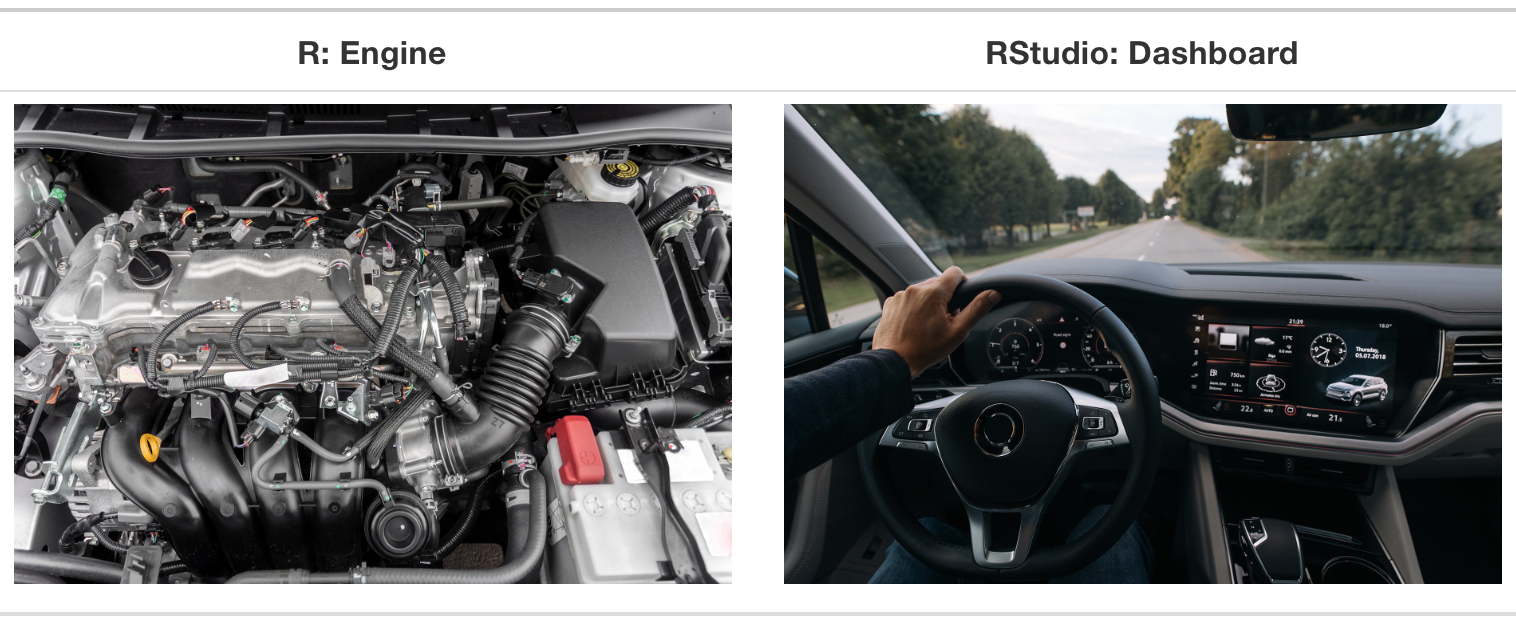
\includegraphics[width=0.95\linewidth]{fig/R_vs_RStudio_1} \caption{Analogy of difference between R and RStudio.}\label{fig:R-vs-RStudio-1}
\end{figure}

More precisely, R is a programming language that runs computations, while RStudio is an \emph{integrated development environment (IDE)} that provides an interface by adding many convenient features and tools. So just as the way of having access to a speedometer, rearview mirrors, and a navigation system makes driving much easier, using RStudio's interface makes using R much easier as well.

Much as we don't drive a car by interacting directly with the engine but rather by interacting with elements on the car's dashboard, we won't be using R directly but rather we will use RStudio's interface. After you install R and RStudio on your computer, you'll have two new \emph{programs} (also called \emph{applications}) you can open. We'll always work in RStudio and not in the R application. Figure \ref{fig:R-vs-RStudio-2a} shows what icon you should be clicking on your computer.

\begin{figure}
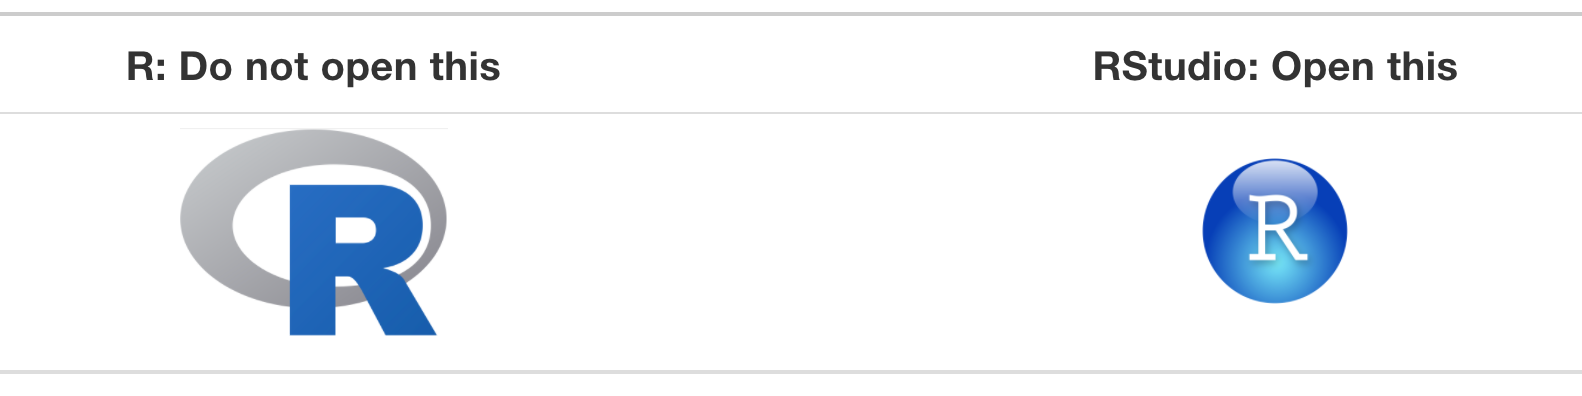
\includegraphics[width=0.9\linewidth]{fig/R_vs_RStudio} \caption{Icons of R versus RStudio on your computer.}\label{fig:R-vs-RStudio-2a}
\end{figure}

After you open RStudio, you should see something similar to Figure \ref{fig:RStudio-interfacea} where three or four panels dividing the screen.

\begin{figure}
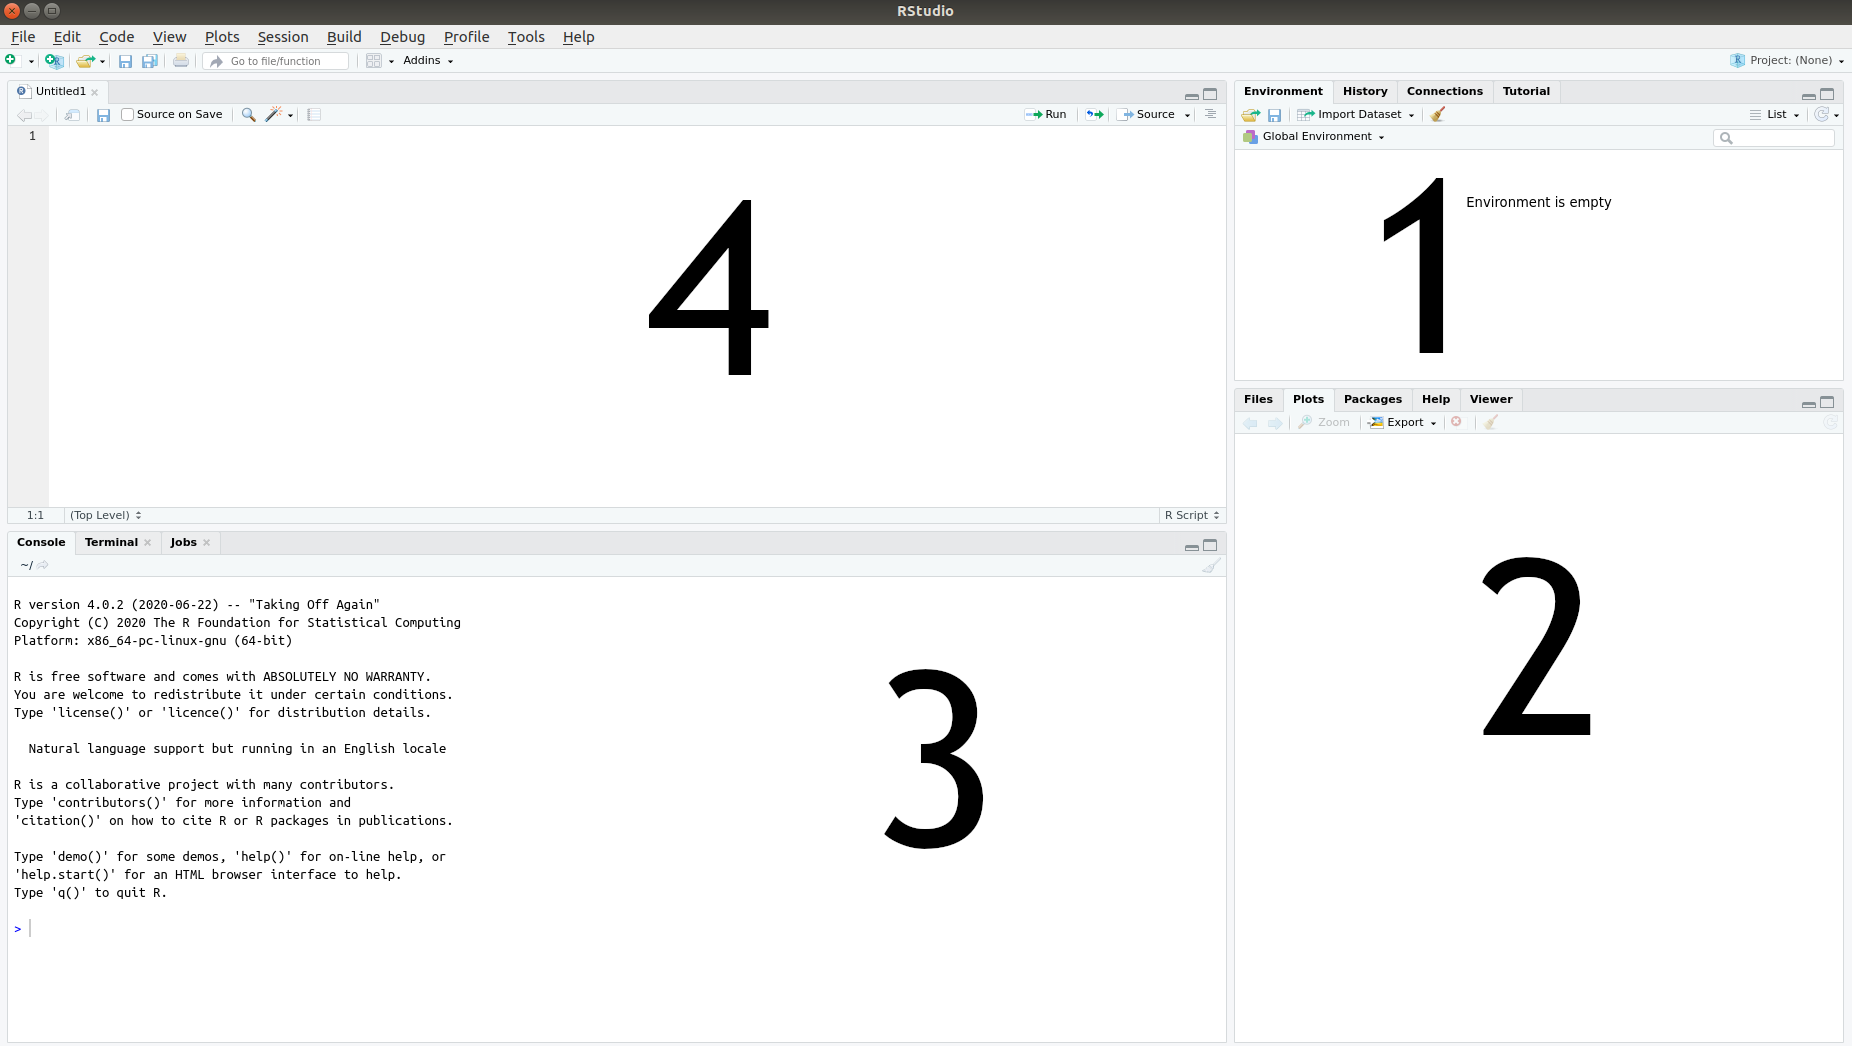
\includegraphics[width=0.93\linewidth]{fig/rstudio2} \caption{RStudio interface to R.}\label{fig:RStudio-interfacea}
\end{figure}

\begin{enumerate}
\def\labelenumi{\arabic{enumi}.}
\tightlist
\item
  The \emph{Environment} panel, where a list of the data you have imported and created can be found.
\item
  The \emph{Files}, \emph{Plots} and \emph{Help} panel, where you can see a list of available files, will be able to view graphs that you produce, and can find help documents for different parts of R.
\item
  The \emph{Console} panel, used for running code. This is where we'll start with the first few examples.
\item
  The \emph{Script} panel, used for writing code. This is where you'll spend most of your time working.
\end{enumerate}

The \emph{Console} panel will contain R's startup message, which shows information about which version of R you're running. My startup message at the time of writing was as follows:

\begin{quote}
R version 4.1.2 (2021-11-01) -- ``Bird Hippie''
Copyright (C) 2021 The R Foundation for Statistical Computing
Platform: x86\_64-pc-linux-gnu (64-bit)

R is free software and comes with ABSOLUTELY NO WARRANTY.
You are welcome to redistribute it under certain conditions.
Type `license()' or `licence()' for distribution details.

Natural language support but running in an English locale

R is a collaborative project with many contributors.
Type `contributors()' for more information and
`citation()' on how to cite R or R packages in publications.

Type `demo()' for some demos, `help()' for on-line help, or
`help.start()' for an HTML browser interface to help.
Type `q()' to quit R.
\end{quote}

If you don't have panel number 4, open it by opening an existing R-script or creating a new one. You can create a new on by clicking \emph{Ctrl+Shift+N} (alternatively, you can use the menu: File\(\rightarrow\)New File\(\rightarrow\)R Script).

You can resize the panels as you like, either by clicking and dragging their borders or using the minimise/maximise buttons in the upper right corner of each panel. Clicking \emph{Ctrl++} and \emph{Ctrl+-} allows to make the fonts larger or smaller.

When you exit RStudio, you will be asked if you wish to \emph{save your workspace}, meaning that the data that you've worked with will be stored so that it is available the next time you run R. That might sound like a good idea, but in general, I recommend that you don't save your workspace, as that often turns out to cause problems down the line. It is almost invariably a much better idea to simply rerun the code you worked with in your next R session.

\hypertarget{how-to-use-r-and-rstudio-without-installation}{%
\section{How to use R and RStudio without installation}\label{how-to-use-r-and-rstudio-without-installation}}

If you don't want to install R on your PC or you don't have admin rights to do so, you can use RStudio online doing \emph{cloud computing} on \url{https://posit.cloud/}.
Posit Cloud (formerly RStudio Cloud) is a cloud-based solution that allows anyone to do, share, teach and learn data science online. It is free for individuals with some restrictions and limited capacities.

\hypertarget{installing}{%
\section{Installing R and RStudio}\label{installing}}

You will first need to download and install both R and RStudio (Desktop version) on your computer. It is important that you install R first and then install RStudio.

\begin{enumerate}
\def\labelenumi{\arabic{enumi}.}
\tightlist
\item
  \textbf{You must do this first:} Download and install R by going to \url{https://cloud.r-project.org/}. \index{R!installation}
\end{enumerate}

\begin{itemize}
\tightlist
\item
  If you are a Windows user: Click on ``Download R for Windows'', then click on ``base'', then click on the Download link.
\item
  If you are macOS user: Click on ``Download R for (Mac) OS X'', then under ``Latest release:'' click on R-X.X.X.pkg, where R-X.X.X is the version number. For example, the latest version of R as of November 25, 2019 was R-3.6.1.
\item
  If you are a Linux user: Click on ``Download R for Linux'' and choose your distribution for more information on installing R for your setup.
\end{itemize}

\begin{enumerate}
\def\labelenumi{\arabic{enumi}.}
\tightlist
\item
  \textbf{You must do this second:} Download and install RStudio at \url{https://www.rstudio.com/products/rstudio/download/}.
\end{enumerate}

\begin{itemize}
\tightlist
\item
  Scroll down to ``Installers for Supported Platforms'' near the bottom of the page.
\item
  Click on the download link corresponding to your computer's operating system.
  \index{RStudio!installation}
\end{itemize}

\hypertarget{packages}{%
\section{What are R packages?}\label{packages}}

A package is basically just a big collection of functions, data sets and other R objects that are all grouped together under a common name. Some packages are already installed when you put R on your computer, but the vast majority of them of R packages are out there on the internet, waiting for you to download, install and use them.
R packages are collections of functions and data sets developed by the community. They increase the power of R by improving existing base R functionalities, or by adding new ones. For example, if you are usually working with data frames, probably you will have heard about \emph{dplyr} or \emph{data.table}, two of the most popular R packages. More than 10,000 packages are available at the official repository (CRAN) and many more are publicly available through the internet.

In this section, I'll describe how to work with packages using the Rstudio tools. Along the way, you'll see that whenever you get Rstudio to do something (e.g., install a package), you'll actually see the R commands that get created.

However, before we get started, there's a critical distinction that you need to understand, which is the difference between having a package \textbf{installed} on your computer, and having a package \textbf{loaded} in R. When you install R on your computer only a small number of packages come bundled with the basic R installation. The installed packages are on your computer. The critical thing to remember is that just because something is on your computer doesn't mean R can use it. In order for R to be able to \emph{use} one of your installed packages, that package must also be \emph{loaded}. Generally, when you open up R, only a few of these packages (about 7 or 8) are actually loaded. Basically what it boils down to is this:

\begin{enumerate}
\def\labelenumi{\arabic{enumi}.}
\tightlist
\item
  A package must be installed before it can be loaded.
\item
  A package must be loaded before it can be used.
\end{enumerate}

We only need to install a package once on our computer. However, to use the package, we need to load the library every time we start a new R environment. You can think of this as installing a bulb versus turning on the light.

\begin{figure}
\centering
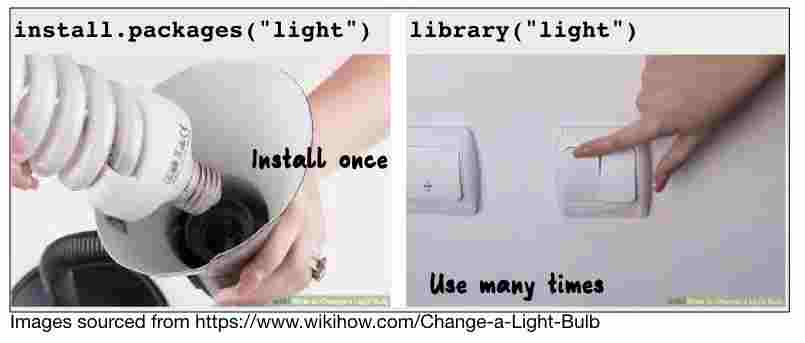
\includegraphics[width=0.5\textwidth,height=\textheight]{fig/lightpackage.jpeg}
\caption{\label{fig:lightpackage} Installing packages}
\end{figure}

The two step process might seem a little odd at first, but the designers of R had very good reasons to do it this way. That is, there are more than 10.000 packages, and probably about 8000 authors of packages, and no-one really knows what all of them do. Keeping the installation separate from the loading minimizes the chances that two packages will interact with each other in a nasty way. Moreover having installed all available packages would probably blow your hard disk.

Another good analogy for R packages \index{R packages} is they are like apps you can download onto a mobile phone:

\begin{figure}
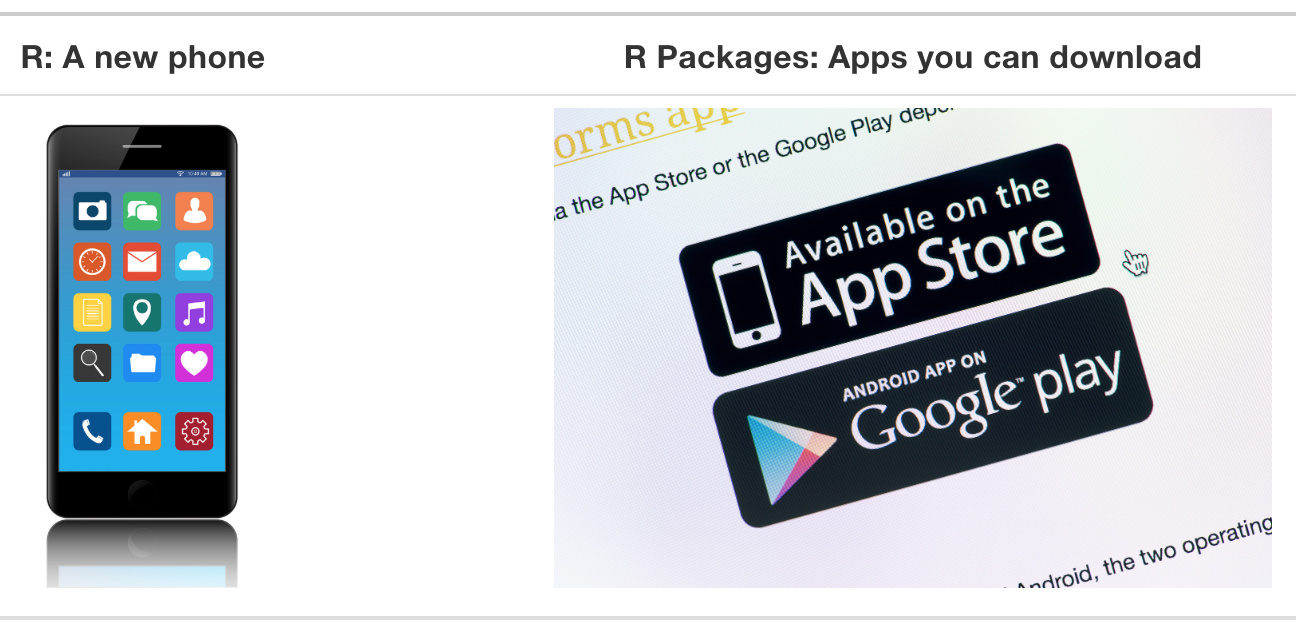
\includegraphics[width=0.7\linewidth]{fig/R_vs_R_packages} \caption{Analogy of R versus R packages.}\label{fig:R-vs-R-packages}
\end{figure}

So R is like a new mobile phone: while it has a certain amount of features when you use it for the first time, it doesn't have everything. R packages are like the apps you can download onto your phone from Apple's App Store or Android's Google Play.

\hypertarget{package-installation}{%
\subsection{Package installation}\label{package-installation}}

There are two ways to install an R package: an easy way and a very easy way. \index{R packages!installation} Let's install the \texttt{ggplot2} package the easy way first as shown in Figure \ref{fig:easy-way-install}. In the Files pane of RStudio:

\begin{enumerate}
\def\labelenumi{\alph{enumi})}
\tightlist
\item
  Click on the ``Packages'' tab.
\item
  Click on ``Install'' next to Update.
\item
  Type the name of the package under ``Packages (separate multiple with space or comma):'' In this case, type \texttt{ggplot2}.
\item
  Click ``Install.''
\end{enumerate}

\begin{figure}
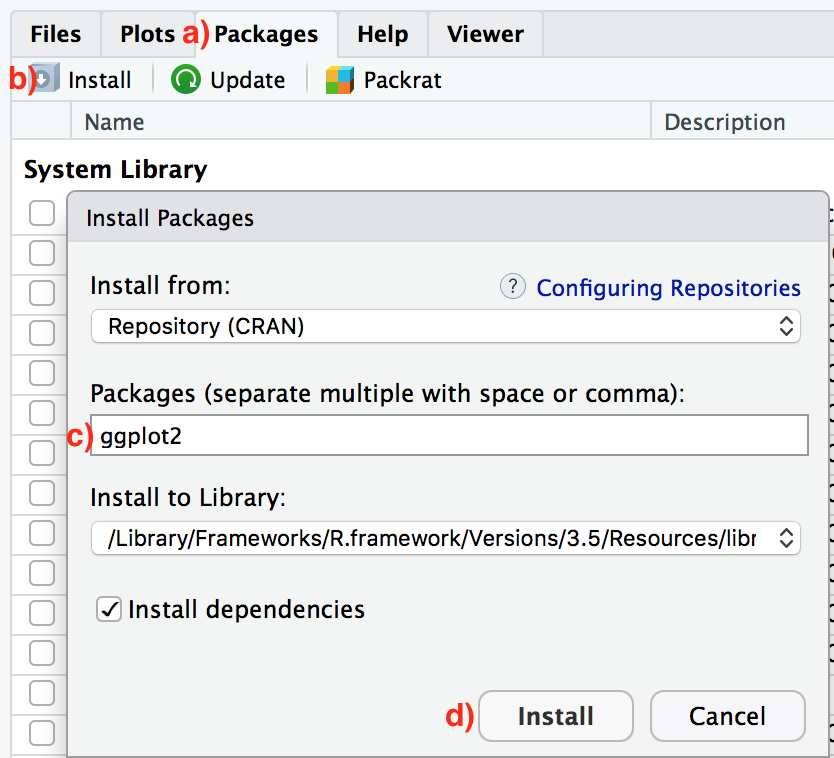
\includegraphics[width=0.55\linewidth,height=0.55\textheight]{fig/install_packages_easy_way} \caption{Installing packages in R the easy way.}\label{fig:easy-way-install}
\end{figure}

An alternative way to install a package is by typing

\begin{Shaded}
\begin{Highlighting}[]
\FunctionTok{install.packages}\NormalTok{(}\StringTok{"ggplot2"}\NormalTok{)}
\end{Highlighting}
\end{Shaded}

in the console pane of RStudio and pressing Return/Enter on your keyboard. Note you must include the quotation marks around the name of the package.

Much like an app on your phone, you only have to install a package once. However, if you want to update a previously installed package to a newer version, you need to reinstall it by repeating the earlier steps.

\hypertarget{package-loading}{%
\subsection{Package loading}\label{package-loading}}

Recall that after you've installed a package, you need to \emph{load it}. In other words, you need to \emph{open it}. We do this by using the \texttt{library()} command. \index{R packages!loading}

For example, to load the \texttt{ggplot2} package, run the following code in the console pane. What do we mean by ``run the following code''? Either type or copy-and-paste the following code into the console pane and then hit the Enter key.

\begin{Shaded}
\begin{Highlighting}[]
\FunctionTok{library}\NormalTok{(}\StringTok{"ggplot2"}\NormalTok{)}
\end{Highlighting}
\end{Shaded}

If after running the earlier code, a blinking cursor returns next to the \texttt{\textgreater{}} ``prompt'' sign, it means you were successful and the \texttt{ggplot2} package is now loaded and ready to use. If, however, you get a red ``error message'' that reads

\begin{verbatim}
Error in library(ggplot2) : there is no package called ‘ggplot2’
\end{verbatim}

It means that you didn't successfully install it. If you get this error message, go back to section \ref{package-installation} on R package installation and make sure to install the \texttt{ggplot2} package before proceeding.

One very common mistake new R users make when wanting to use particular packages is they forget to \emph{load} them first by using the \texttt{library()} command we just saw. Remember: \emph{you have to load each package you want to use every time you start RStudio.} If you don't first \emph{load} a package, but attempt to use one of its features, you'll see an error message similar to:

\begin{verbatim}
Error: could not find function
\end{verbatim}

This is a different error message than the one you just saw on a package not having been installed yet. R is telling you that you are trying to use a function in a package that has not yet been \emph{loaded}. R doesn't know where to find the function you are using. Almost all new users forget to do this when starting out, and it is a little annoying to get used to doing it. However, you'll remember with practice and after some time it will become second nature for you.

\hypertarget{dont-do-it}{%
\section{Don't do it}\label{dont-do-it}}

There are many conventions, rules and specific things that you should know better in order not to get into trouble with R so easily. It is tedious to explain all these dos and don'ts in detail, so please obey. It will make your life with R easier. I assure you, will understand later on why it is beneficial to follow these suggested conventions. So here is a non-exhaustive list of things to know:

\textbf{Don't\ldots{}}

\begin{itemize}
\tightlist
\item
  Don't forget that R programming language is case sensitive.
\item
  Don't name objects such as vectors, numbers, variables, and data frames with a starting number.
\item
  Don't use dots in names of objects.
\item
  Don't use certain keywords in naming objects, such as if, else, repeat, while, function, for, in, next, break, TRUE, FALSE, NULL, Inf, NaN, and NA.
\item
  Don't use backslash \texttt{\textbackslash{}} for navigating the file system; use front slash \texttt{/} instead.
\item
  Don't use whitespace and indentation for naming files, directories, or objects.
\item
  Don't ignore warnings or errors unless you know what they mean.
\item
  Don't use hard-coded values; instead, define objects to represent these values.
\item
  Don't forget to (install and) load packages that contain functions you want to use.
\item
  Don't forget to set your working directory.
\item
  Don't forget to comment your code.
\item
  Don't use \texttt{=}, for assignment but \texttt{\textless{}-}.
\end{itemize}

An exhaustive style guide on how to write code can be found here: \url{https://style.tidyverse.org}

\hypertarget{swirl}{%
\chapter{Learn interactively with swirl}\label{swirl}}

The R package \emph{swirl} makes it fun and easy to learn R programming and data science.
\emph{swirl} teaches you R programming and data science interactively, at your own pace,
and right in the R console! You get immediate feedback on your progress.
If you are new to R, have no fear. \emph{swirl} will walk you through each of the steps
required to employ Rstudio and R for your purpose.
To start it, please follow my instructions precisely!

Open Rstudio and type in the console the following:

\begin{Shaded}
\begin{Highlighting}[]
\FunctionTok{install.packages}\NormalTok{(}\StringTok{"swirl"}\NormalTok{)}
\FunctionTok{library}\NormalTok{(}\StringTok{"swirl"}\NormalTok{)}
\FunctionTok{ls}\NormalTok{()}
\FunctionTok{rm}\NormalTok{(}\AttributeTok{list=}\FunctionTok{ls}\NormalTok{())}
\FunctionTok{install\_course\_github}\NormalTok{(}\StringTok{"hubchev"}\NormalTok{, }\StringTok{"swirl{-}it"}\NormalTok{)}
\FunctionTok{swirl}\NormalTok{()}
\end{Highlighting}
\end{Shaded}

The above lines of code do the following:

\begin{itemize}
\tightlist
\item
  Install the \emph{swirl} package.
\item
  Load the \emph{swirl} package.
\item
  List the content of the environment.
\item
  Remove everything from the environment.
\item
  Install my \emph{swirl} course that is hosted on GitHub.
\item
  With \emph{swirl} you start \emph{swirl} and your learning experience.
\end{itemize}

If the course has failed to install, you can try to download the file \texttt{swirl-it.swc} from \url{https://github.com/hubchev/swirl-it} and install the course with loading the swirl package and typing \texttt{install\_course()} into the console.

Please choose the course \emph{swirl-it} and the learning module \emph{huber-intro-1}.
You can exit \emph{swirl} at any time by typing \texttt{bye()} or by clicking the \emph{Esc} on your keyboard.

After you have successfully finished learning module \emph{huber-intro-1} please go ahead with the learning module \emph{huber-intro-2} that is also part of my swirl course \emph{swirl-it}.

\hypertarget{swirl-modules-on-data-analytical-basics}{%
\subsubsection*{\texorpdfstring{\emph{swirl} modules on data analytical basics}{swirl modules on data analytical basics}}\label{swirl-modules-on-data-analytical-basics}}

In my swirl modules \emph{huber-data-1}, \emph{huber-data-2}, and \emph{huber-data-3} I introduce some very basic statistical principles on how to analyse data.

\hypertarget{swirl-module-on-the-tidyverse-package}{%
\subsubsection*{\texorpdfstring{\emph{swirl} module on the \texttt{tidyverse} package}{swirl module on the tidyverse package}}\label{swirl-module-on-the-tidyverse-package}}

I compiled a short \emph{swirl} module to introduce the \emph{tidyverse} universe. This is a powerful collection of packages which I discuss later on. The learning module is also part of my \emph{swirl-it} course.

\hypertarget{other-swirl-modules}{%
\subsubsection*{\texorpdfstring{Other \emph{swirl} modules}{Other swirl modules}}\label{other-swirl-modules}}

You can also install some other courses. You find a list of courses here \url{http://swirlstats.com/scn/index.html} or here \url{https://github.com/swirldev/swirl_courses}.

I recommend this one as it gives a general overview on very basic principles of R:

\begin{Shaded}
\begin{Highlighting}[]
\FunctionTok{library}\NormalTok{(swirl)}
\FunctionTok{install\_course\_github}\NormalTok{(}\StringTok{"swirldev"}\NormalTok{, }\StringTok{"R\_Programming\_E"}\NormalTok{)}
\FunctionTok{swirl}\NormalTok{()}
\end{Highlighting}
\end{Shaded}

\hypertarget{how-to-work-with-r-scripts}{%
\chapter{How to work with R scripts}\label{how-to-work-with-r-scripts}}

\hypertarget{r-scripts-why-they-are-useful}{%
\section{R Scripts: Why they are useful}\label{r-scripts-why-they-are-useful}}

Typing functions into the console to run code may seem simple, but this interactive style has limitations:

\begin{itemize}
\tightlist
\item
  Typing commands one at a time can be cumbersome and time-consuming.
\item
  It's hard to save your work effectively.
\item
  Going back to the beginning when you make a mistake is annoying.
\item
  You can't leave notes for yourself.
\item
  Reusing and adapting analyses can be difficult.
\item
  It's hard to do anything except the basics.
\item
  Sharing your work with others can be challenging.
\end{itemize}

That's where having a transcript of all the code, which can be re-run and edited at any time, becomes useful. An R script is precisely that - a plain text file that contains code and comments and this comes with advantages:

\begin{itemize}
\tightlist
\item
  Scripts provide a record of everything you did during your data analysis.
\item
  You can easily edit and re-run code in a script.
\item
  Scripts allow you to leave notes for yourself.
\item
  Scripts make it easy to reuse and adapt analyses.
\item
  Scripts allow you to do more complex analyses.
\item
  Scripts make it easy to share your work with others.
\end{itemize}

\hypertarget{generate-write-and-run-r-scripts}{%
\section{Generate, write and run R scripts}\label{generate-write-and-run-r-scripts}}

To \textbf{generate a script} you can

\begin{enumerate}
\def\labelenumi{\arabic{enumi}.}
\tightlist
\item
  Go to the \emph{File} menu, select \emph{New File} and then choose \emph{R Script} or
\item
  Use the keyboard shortcut \emph{Ctrl+Shift+N} (Windows) or \emph{Cmd+Shift+N} (Mac) or
\item
  Type the following command in the Console:
\end{enumerate}

\begin{Shaded}
\begin{Highlighting}[]
\FunctionTok{file.create}\NormalTok{(}\StringTok{"hello.R"}\NormalTok{)}
\end{Highlighting}
\end{Shaded}

In the first two ways, a new R script window will open which can be edited and should be saved either by clicking on the \emph{File} menu and selecting \emph{Save}, clicking the disk icon, or by using the shortcut \emph{Ctrl+S} (Windows) or \emph{Cmd+S} (Mac).
If you go for the third way, you need to open it manually.

Regardless of your preferred way of generating a script, we can now start \textbf{writing} our first script:

\begin{Shaded}
\begin{Highlighting}[]
\FunctionTok{setwd}\NormalTok{(}\StringTok{"/home/sthu/Dropbox/hsf/23{-}ss/ds/"}\NormalTok{)}
\NormalTok{x }\OtherTok{\textless{}{-}} \StringTok{"hello world"}
\FunctionTok{print}\NormalTok{(x)}
\end{Highlighting}
\end{Shaded}

\begin{verbatim}
## [1] "hello world"
\end{verbatim}

Then save the script using the menus (File \textgreater{} Save) as hello.R.

The above lines of code do the following:

\begin{itemize}
\tightlist
\item
  \texttt{setwd()} allows to set the working directory. If you are not familiar with file systems, please read section \ref{sec:navigation} in the appendix.
\item
  With the assignment operator \texttt{\textless{}-} we create an object that stores the words ``hello world'' in an object entitled \texttt{x}. In the next section \ref{sec:assignmentoper} the assignment operator is further explained.
\item
  With the third input we print the content of the object \texttt{x}.
\end{itemize}

So how do we \textbf{run the script}? Assuming that the \texttt{hello.R} file has been saved to your working directory, then you can run the script using the following command:

\begin{Shaded}
\begin{Highlighting}[]
\FunctionTok{source}\NormalTok{( }\StringTok{"hello.R"}\NormalTok{ )}
\end{Highlighting}
\end{Shaded}

Suppose you saved the script in a sub-folder called \texttt{scripts} of your working directory, then you need to run the script using the following command:

\begin{Shaded}
\begin{Highlighting}[]
\FunctionTok{source}\NormalTok{(}\StringTok{"./scripts/hello.R"}\NormalTok{) }
\end{Highlighting}
\end{Shaded}

Just note that the dot, \texttt{.}, means the current folder.
Instead of using the \texttt{source} function, you can click on the \texttt{source} button in Rstudio.

With the character \texttt{\#} you can write a comment in a script and R will simply ignore everything that follows in that line onwards.

\hypertarget{sec:assignmentoper}{%
\section{\texorpdfstring{The assignment operator: \texttt{\textless{}-}}{The assignment operator: \textless-}}\label{sec:assignmentoper}}

Suppose I'm trying to calculate how much money I'm going to make from this book. I agree, it is an unrealistic example but it will help you to understand R.
Let's assume I'm only going to sell 350 copies. To create a variable called \texttt{sales} and assigns a value to it, we need to use the \emph{assignment operator} of R, which is \texttt{\textless{}-} as follows:

\begin{Shaded}
\begin{Highlighting}[]
\NormalTok{sales }\OtherTok{\textless{}{-}} \DecValTok{350}
\end{Highlighting}
\end{Shaded}

When you hit enter, R doesn't print out any output. If you are using Rstudio, and the \emph{environment panel} you can see that something happened there, can you? It just gives you another command prompt. However, behind the scenes R has created a variable called \texttt{sales} and given it a value of \texttt{350}. You can check that this has happened by asking R to print the variable on screen. And the simplest way to do that is to type the name of the variable and hit enter.

\begin{Shaded}
\begin{Highlighting}[]
\NormalTok{sales}
\end{Highlighting}
\end{Shaded}

\begin{verbatim}
## [1] 350
\end{verbatim}

Worth a mentioning is the curious features of R that there are several different ways of making assignments. In addition to the \texttt{\textless{}-} operator, we can also use \texttt{-\textgreater{}} and \texttt{=}. If you want to use \texttt{-\textgreater{}}, you might expect from just looking at the symbol you should write it like this:

\begin{Shaded}
\begin{Highlighting}[]
\DecValTok{350} \OtherTok{{-}\textgreater{}}\NormalTok{ sales}
\end{Highlighting}
\end{Shaded}

However, it is common practice to use \texttt{\textless{}-} and I recommend only to use this one because it is easier to read in scripts.

\hypertarget{doing-calculation-in-scripts}{%
\section{Doing calculation in scripts}\label{doing-calculation-in-scripts}}

R can do any kind of arithmetic calculation with the arithmetic operators given in the table below. Using the assignment operator, R functions, and the features of a R script is easy and gives an idea how R works and how you should embrace the power of the programming language.

\begin{longtable}[]{@{}lccc@{}}
\toprule()
operation & operator & example input & example output \\
\midrule()
\endhead
addition & + & 10+2 & 12 \\
subtraction & - & 9-3 & 6 \\
multiplication & * & 5*5 & 25 \\
division & / & 10/3 & 3 \\
power & \texttt{\^{}} & 5\^{}2 & 25 \\
\bottomrule()
\end{longtable}

So please copy and past the following lines of code into a R script of yours, try to run it on your PC, and try to understand it. Of course, you have to tweak the script a bit to make it run on your PC. For example, I doubt you have the same working directory that I decided to use.

\begin{Shaded}
\begin{Highlighting}[]
\CommentTok{\# Set working directory}
\FunctionTok{setwd}\NormalTok{(}\StringTok{"\textasciitilde{}/Dropbox/hsf/23{-}ss/ds"}\NormalTok{)}
\CommentTok{\# Create a vector that contains the sales data}
\NormalTok{sales\_by\_month }\OtherTok{\textless{}{-}} \FunctionTok{c}\NormalTok{(}\DecValTok{0}\NormalTok{, }\DecValTok{100}\NormalTok{, }\DecValTok{200}\NormalTok{, }\DecValTok{50}\NormalTok{, }\DecValTok{3}\NormalTok{, }\DecValTok{4}\NormalTok{, }\DecValTok{8}\NormalTok{, }\DecValTok{0}\NormalTok{, }\DecValTok{0}\NormalTok{, }\DecValTok{0}\NormalTok{, }\DecValTok{0}\NormalTok{, }\DecValTok{0}\NormalTok{)}
\NormalTok{sales\_by\_month}
\NormalTok{sales\_by\_month[}\DecValTok{2}\NormalTok{]}
\NormalTok{sales\_by\_month[}\DecValTok{4}\NormalTok{]}
\NormalTok{february\_sales }\OtherTok{\textless{}{-}}\NormalTok{ sales\_by\_month[}\DecValTok{2}\NormalTok{]}
\NormalTok{february\_sales}
\NormalTok{sales\_by\_month[}\DecValTok{5}\NormalTok{] }\OtherTok{\textless{}{-}} \DecValTok{25} \CommentTok{\# added May sales data}
\NormalTok{sales\_by\_month}
\CommentTok{\# Do I have 12 month?}
\FunctionTok{length}\NormalTok{( }\AttributeTok{x =}\NormalTok{ sales\_by\_month )}
\CommentTok{\# Assume each unit costs 7 Euro, then the revenue is}
\NormalTok{price }\OtherTok{\textless{}{-}} \DecValTok{7}
\NormalTok{revenue }\OtherTok{\textless{}{-}}\NormalTok{ sales\_by\_month}\SpecialCharTok{*}\NormalTok{price}
\NormalTok{revenue}
\CommentTok{\# To get statistics for daily revenue we define the number of days:}
\NormalTok{days\_per\_month }\OtherTok{\textless{}{-}} \FunctionTok{c}\NormalTok{(}\DecValTok{31}\NormalTok{, }\DecValTok{28}\NormalTok{, }\DecValTok{31}\NormalTok{, }\DecValTok{30}\NormalTok{, }\DecValTok{31}\NormalTok{, }\DecValTok{30}\NormalTok{, }\DecValTok{31}\NormalTok{, }\DecValTok{31}\NormalTok{, }\DecValTok{30}\NormalTok{, }\DecValTok{31}\NormalTok{, }\DecValTok{30}\NormalTok{, }\DecValTok{31}\NormalTok{)}
\CommentTok{\# Calculate the daily revenue}
\NormalTok{revenue\_per\_day }\OtherTok{\textless{}{-}}\NormalTok{ revenue}\SpecialCharTok{/}\NormalTok{days\_per\_month}
\NormalTok{revenue\_per\_day }
\CommentTok{\# round number }
\FunctionTok{round}\NormalTok{(revenue\_per\_day) }
\end{Highlighting}
\end{Shaded}

Use the ``\texttt{?}'' to search for the documentation of all functions used. In particular, do you understand how the function \texttt{round()} works? What arguments does the function contain? How can you manipulate the pre-defined arguments. For example, can you calculate the rounded revenue per day with two or four digits? Try it out!

\begin{Shaded}
\begin{Highlighting}[]
\NormalTok{?}\FunctionTok{round}\NormalTok{()}
\end{Highlighting}
\end{Shaded}

\hypertarget{sec:generics}{%
\section{User-defined functions}\label{sec:generics}}

One of the great strengths of R is the user's ability to add functions. Sometimes there is a small task (or series of tasks) you need done and you find yourself having to repeat it multiple times. In these types of situations it can be helpful to create your own custom function. The structure of a function is given below:

\begin{Shaded}
\begin{Highlighting}[]
\NormalTok{name\_of\_function }\OtherTok{\textless{}{-}} \ControlFlowTok{function}\NormalTok{(argument1, argument2) \{}
\NormalTok{    statements or code that does something}
    \FunctionTok{return}\NormalTok{(something)}
\NormalTok{\}}
\end{Highlighting}
\end{Shaded}

First you give your function a name.
Then you assign value to it, where the value is the function.
When defining the function you will want to provide the list of arguments required (inputs and/or options to modify behavior of the function), and wrapped between curly brackets place the tasks that are being executed on/using those arguments. The argument(s) can be any type of object (like a scalar, a matrix, a dataframe, a vector, a logical, etc), and it's not necessary to define what it is in any way.
Finally, you can return the value of the object from the function, meaning pass the value of it into the global environment. The important idea behind functions is that objects that are created within the function are local to the environment of the function -- they don't exist outside of the function. Note, a function doesn't require any arguments.

Let's try creating a simple example function. This function will take in a numeric value as input, and return the squared value.

\begin{Shaded}
\begin{Highlighting}[]
\NormalTok{square\_it }\OtherTok{\textless{}{-}} \ControlFlowTok{function}\NormalTok{(x) \{ }
\NormalTok{   square }\OtherTok{\textless{}{-}}\NormalTok{ x }\SpecialCharTok{*}\NormalTok{ x}
   \FunctionTok{return}\NormalTok{(square)}
\NormalTok{\} }
\end{Highlighting}
\end{Shaded}

Now, we can use the function as we would any other function. We type out the name of the function, and inside the parentheses we provide a numeric value \texttt{x}:

\begin{Shaded}
\begin{Highlighting}[]
\FunctionTok{square\_it}\NormalTok{(}\DecValTok{5}\NormalTok{)}
\end{Highlighting}
\end{Shaded}

\begin{verbatim}
## [1] 25
\end{verbatim}

Let us get back to script with sales and try to calculate the monthly growth rates of revenue using a self-written function.

The formula of a growth rate is clear:

\[ g=\left(\frac{y_t-y_{t-1}}{y_{t-1}}\right)\cdot 100=\left(\frac{y_t}{y_{t-1}}-1\right)\cdot 100 \]

So the challenge is to divide the value of \texttt{revenue} with the value of the previous period, a.k.a. the lagged value. Let us assume that the function \texttt{lag()} can give you exactly that value of a vector. Lets try it out:

\begin{Shaded}
\begin{Highlighting}[]
\FunctionTok{lag}\NormalTok{(revenue)}
\end{Highlighting}
\end{Shaded}

\begin{verbatim}
##  [1]   NA    0  700 1400  350  175   28   56    0    0    0
## [12]    0
\end{verbatim}

\begin{Shaded}
\begin{Highlighting}[]
\NormalTok{(revenue}\SpecialCharTok{/}\FunctionTok{lag}\NormalTok{(revenue)}\SpecialCharTok{{-}}\DecValTok{1}\NormalTok{)}\SpecialCharTok{*}\DecValTok{100} 
\end{Highlighting}
\end{Shaded}

\begin{verbatim}
##  [1]   NA  Inf  100  -75  -50  -84  100 -100  NaN  NaN  NaN
## [12]  NaN
\end{verbatim}

Unfortunately, this does not work out. The \texttt{lag()} function does not work as we think it should. Well, the reason is simply that we are using the wrong function. The current \texttt{lag()} function is part of the stats package which is part of R base and is always loaded. The \texttt{lag()} function we aim to use stems from the dplyr package which we must install and load to be able to use it. So let's do it:

\begin{Shaded}
\begin{Highlighting}[]
\CommentTok{\# check if the package is installed}
\FunctionTok{find.package}\NormalTok{(}\StringTok{"dplyr"}\NormalTok{)}
\end{Highlighting}
\end{Shaded}

\begin{verbatim}
## [1] "/home/sthu/R/x86_64-pc-linux-gnu-library/4.2/dplyr"
\end{verbatim}

\begin{Shaded}
\begin{Highlighting}[]
\CommentTok{\# I already installed the package so I can just load it}
\CommentTok{\# install.packages("dplyr")}
\FunctionTok{library}\NormalTok{(}\StringTok{"dplyr"}\NormalTok{)}
\end{Highlighting}
\end{Shaded}

Now, we was informed that among other functions the \texttt{lag()} function is \emph{masked}. That means that now the function of the newly loaded package is active. So, let's try again:

\begin{Shaded}
\begin{Highlighting}[]
\FunctionTok{lag}\NormalTok{(revenue)}
\end{Highlighting}
\end{Shaded}

\begin{verbatim}
##  [1]   NA    0  700 1400  350  175   28   56    0    0    0
## [12]    0
\end{verbatim}

\begin{Shaded}
\begin{Highlighting}[]
\NormalTok{(revenue}\SpecialCharTok{/}\FunctionTok{lag}\NormalTok{(revenue)}\SpecialCharTok{{-}}\DecValTok{1}\NormalTok{)}\SpecialCharTok{*}\DecValTok{100} 
\end{Highlighting}
\end{Shaded}

\begin{verbatim}
##  [1]   NA  Inf  100  -75  -50  -84  100 -100  NaN  NaN  NaN
## [12]  NaN
\end{verbatim}

That looks good now. And here is a way to calculate growth rates with a self-written function:

\begin{Shaded}
\begin{Highlighting}[]
\NormalTok{growth\_rate }\OtherTok{\textless{}{-}} \ControlFlowTok{function}\NormalTok{(x)(x}\SpecialCharTok{/}\FunctionTok{lag}\NormalTok{(x)}\SpecialCharTok{{-}}\DecValTok{1}\NormalTok{)}\SpecialCharTok{*}\DecValTok{100} 
\FunctionTok{growth\_rate}\NormalTok{(revenue)}
\end{Highlighting}
\end{Shaded}

\begin{verbatim}
##  [1]   NA  Inf  100  -75  -50  -84  100 -100  NaN  NaN  NaN
## [12]  NaN
\end{verbatim}

\begin{Shaded}
\begin{Highlighting}[]
\NormalTok{sales\_gr\_rate }\OtherTok{\textless{}{-}} \FunctionTok{growth\_rate}\NormalTok{(revenue)}
\NormalTok{sales\_gr\_rate}
\end{Highlighting}
\end{Shaded}

\begin{verbatim}
##  [1]   NA  Inf  100  -75  -50  -84  100 -100  NaN  NaN  NaN
## [12]  NaN
\end{verbatim}

You know, all functions in R are user-written and sometimes it happens that two people had the idea to name functions identically. In such a case we have to deal with that conflict as we cannot use both functions at the same time. Also, it is a very realistic case that you find a solution somewhere that should work out your problem but you fail to make it run. In such a case it is often a forgotten package that needs to be loaded.

\begin{exercise}
\protect\hypertarget{exr:growthrate}{}\label{exr:growthrate}All roads lead to R(ome)

If you ask ten programmers to solve a particular problem, you will probably receive ten different soltuions that are all valid. R is no exception here. This can be very confussing when just started to learn R.

Below you find two more ways to calculate the a growth rate. Do you understand them?
\end{exercise}

\begin{Shaded}
\begin{Highlighting}[]
\FunctionTok{c}\NormalTok{(}\ConstantTok{NA}\NormalTok{, }\FunctionTok{diff}\NormalTok{(revenue)}\SpecialCharTok{/}\FunctionTok{head}\NormalTok{(revenue, }\SpecialCharTok{{-}}\DecValTok{1}\NormalTok{))}\SpecialCharTok{*}\DecValTok{100}        
\end{Highlighting}
\end{Shaded}

\begin{verbatim}
##  [1]   NA  Inf  100  -75  -50  -84  100 -100  NaN  NaN  NaN
## [12]  NaN
\end{verbatim}

\begin{Shaded}
\begin{Highlighting}[]
\NormalTok{(revenue}\SpecialCharTok{/}\FunctionTok{c}\NormalTok{(}\ConstantTok{NA}\NormalTok{,revenue[}\SpecialCharTok{{-}}\FunctionTok{length}\NormalTok{(revenue)])}\SpecialCharTok{{-}}\DecValTok{1}\NormalTok{)}\SpecialCharTok{*}\DecValTok{100}
\end{Highlighting}
\end{Shaded}

\begin{verbatim}
##  [1]   NA  Inf  100  -75  -50  -84  100 -100  NaN  NaN  NaN
## [12]  NaN
\end{verbatim}

\hypertarget{how-to-manage-data}{%
\chapter{How to manage data}\label{how-to-manage-data}}

\hypertarget{the-tidyverse-universe}{%
\section{The tidyverse universe}\label{the-tidyverse-universe}}

If you want to work with R, you should get known to the \emph{tidyverse} package. The tidyverse is an opinionated collection of R packages designed for data science. All packages share an underlying design philosophy, grammar, and data structures.
The core packages are ggplot2, dplyr, tidyr, readr, purrr, tibble, stringr, and forcats, which provide functionality to model, transform, and visualize data. An additional 12 packages assist the core. As of November 2018, the tidyverse package and some of its individual packages comprise 5 out of the top 10 most downloaded R packages. The tidyverse is the subject of multiple books and papers and \citet{Wickham2023R} is all about it. Thus, read sections 3 (\href{https://r4ds.hadley.nz/workflow-basics.html}{Workflow: basics}) and 4 (\href{https://r4ds.hadley.nz/data-transform.html}{Data transformation}) of \citet{Wickham2023R}, visit the website www.tidyverse.org, and, if you still haven`t done, do the tidyverse module of my swirl package, called \emph{swirl-it}.

Install the complete tidyverse with:

\begin{Shaded}
\begin{Highlighting}[]
    \FunctionTok{install.packages}\NormalTok{(}\StringTok{"tidyverse"}\NormalTok{)}
\end{Highlighting}
\end{Shaded}

\hypertarget{the-pipe-operator}{%
\section{The pipe operator}\label{the-pipe-operator}}

The pipe operator, \%\textgreater\%, comes from the magrittr package which is also a part of the tidyverse package. The \emph{base} pipe operator, \textbar\textgreater, is since R.4.1.0 part of base R. For most cases these two are identical. The pipe is to help you write code in a way that is easier to read and understand.
As R is a functional language, code often contains a lot of parenthesis, ( and ). Nesting those parentheses together is complex and you easily get lost. This makes your R code hard to read and understand. Here's where \%\textgreater\% comes in to the rescue! Consider the following chunk of code to explain the usage of the pipe:

\begin{Shaded}
\begin{Highlighting}[]
\CommentTok{\# create some data \textasciigrave{}x\textasciigrave{}}
\NormalTok{x }\OtherTok{\textless{}{-}} \FunctionTok{c}\NormalTok{(}\FloatTok{0.109}\NormalTok{, }\FloatTok{0.359}\NormalTok{, }\FloatTok{0.63}\NormalTok{, }\FloatTok{0.996}\NormalTok{, }\FloatTok{0.515}\NormalTok{, }\FloatTok{0.142}\NormalTok{, }\FloatTok{0.017}\NormalTok{, }\FloatTok{0.829}\NormalTok{, }\FloatTok{0.907}\NormalTok{)}
\NormalTok{x}
\end{Highlighting}
\end{Shaded}

\begin{verbatim}
## [1] 0.109 0.359 0.630 0.996 0.515 0.142 0.017 0.829 0.907
\end{verbatim}

\begin{Shaded}
\begin{Highlighting}[]
\CommentTok{\# take the logarithm of \textasciigrave{}x\textasciigrave{}, }
\NormalTok{x2 }\OtherTok{\textless{}{-}} \FunctionTok{log}\NormalTok{(x)}
\NormalTok{x2}
\end{Highlighting}
\end{Shaded}

\begin{verbatim}
## [1] -2.216407397 -1.024432890 -0.462035460 -0.004008021
## [5] -0.663588378 -1.951928221 -4.074541935 -0.187535124
## [9] -0.097612829
\end{verbatim}

\begin{Shaded}
\begin{Highlighting}[]
\CommentTok{\# compute the lagged and iterated differences (see \textasciigrave{}diff()\textasciigrave{})}
\NormalTok{x3 }\OtherTok{\textless{}{-}} \FunctionTok{diff}\NormalTok{(x2)}
\NormalTok{x3}
\end{Highlighting}
\end{Shaded}

\begin{verbatim}
## [1]  1.19197451  0.56239743  0.45802744 -0.65958036
## [5] -1.28833984 -2.12261371  3.88700681  0.08992229
\end{verbatim}

\begin{Shaded}
\begin{Highlighting}[]
\CommentTok{\#  Make yourself familiar with the functions round() and round the result (1 digit)}
\NormalTok{x4 }\OtherTok{\textless{}{-}} \FunctionTok{round}\NormalTok{(x3, }\DecValTok{1}\NormalTok{)}
\NormalTok{x4}
\end{Highlighting}
\end{Shaded}

\begin{verbatim}
## [1]  1.2  0.6  0.5 -0.7 -1.3 -2.1  3.9  0.1
\end{verbatim}

That is rather long and we actually don't need objects x2, x3, and x4. Well, then let us write that in a nested function:

\begin{Shaded}
\begin{Highlighting}[]
\NormalTok{x }\OtherTok{\textless{}{-}} \FunctionTok{c}\NormalTok{(}\FloatTok{0.109}\NormalTok{, }\FloatTok{0.359}\NormalTok{, }\FloatTok{0.63}\NormalTok{, }\FloatTok{0.996}\NormalTok{, }\FloatTok{0.515}\NormalTok{, }\FloatTok{0.142}\NormalTok{, }\FloatTok{0.017}\NormalTok{, }\FloatTok{0.829}\NormalTok{, }\FloatTok{0.907}\NormalTok{)}

\FunctionTok{round}\NormalTok{(}\FunctionTok{diff}\NormalTok{(}\FunctionTok{log}\NormalTok{(x)), }\DecValTok{1}\NormalTok{)}
\end{Highlighting}
\end{Shaded}

\begin{verbatim}
## [1]  1.2  0.6  0.5 -0.7 -1.3 -2.1  3.9  0.1
\end{verbatim}

This is short but you easily loose overview. The solution is the \emph{pipe}:

\begin{Shaded}
\begin{Highlighting}[]
\CommentTok{\# load one of these packages: \textasciigrave{}magrittr\textasciigrave{} or \textasciigrave{}tidyverse\textasciigrave{}}
\FunctionTok{library}\NormalTok{(tidyverse)}

\CommentTok{\# Perform the same computations on \textasciigrave{}x\textasciigrave{} as above}
\NormalTok{x }\SpecialCharTok{\%\textgreater{}\%} \FunctionTok{log}\NormalTok{() }\SpecialCharTok{\%\textgreater{}\%}
    \FunctionTok{diff}\NormalTok{() }\SpecialCharTok{\%\textgreater{}\%}
    \FunctionTok{round}\NormalTok{(}\DecValTok{1}\NormalTok{)}
\end{Highlighting}
\end{Shaded}

\begin{verbatim}
## [1]  1.2  0.6  0.5 -0.7 -1.3 -2.1  3.9  0.1
\end{verbatim}

You can read the \%\textgreater\% with ``and then'' because it takes the results of some function ``and then'' does something with that in the next.
Another example can be found in this short clip: \href{https://youtu.be/PX5NuteZ3Vg}{Using the pipe operator in R}

Read out loud the following code:

\begin{Shaded}
\begin{Highlighting}[]
\FunctionTok{library}\NormalTok{(}\StringTok{"datasets"}\NormalTok{)}
\NormalTok{iris }\SpecialCharTok{\%\textgreater{}\%}
  \FunctionTok{subset}\NormalTok{(Sepal.Length }\SpecialCharTok{\textgreater{}} \DecValTok{5}\NormalTok{) }\SpecialCharTok{\%\textgreater{}\%}
  \FunctionTok{aggregate}\NormalTok{(. }\SpecialCharTok{\textasciitilde{}}\NormalTok{ Species , . , mean)}
\end{Highlighting}
\end{Shaded}

\begin{verbatim}
##      Species Sepal.Length Sepal.Width Petal.Length
## 1     setosa     5.313636    3.713636     1.509091
## 2 versicolor     5.997872    2.804255     4.317021
## 3  virginica     6.622449    2.983673     5.573469
##   Petal.Width
## 1   0.2772727
## 2   1.3468085
## 3   2.0326531
\end{verbatim}

A solution may be the following: ``you take the Iris data \emph{and then} you subset the data \emph{and then} you aggregate the data and show the mean''.

\hypertarget{data-manipulation-with-dplyr}{%
\section{Data manipulation with dplyr}\label{data-manipulation-with-dplyr}}

The dplyr package, which is part of tidyverse, make data manipulation easy:
- Pick observations by their values (\texttt{filter()}).
- Reorder the rows (\texttt{arrange()}).
- Pick variables by their names (\texttt{select()}).
- Create new variables with functions of existing variables
(\texttt{mutate()}).
- Collapse many values down to a single summary (\texttt{summarise()}).

These functions can all be used in conjunction with \texttt{group\_by()} , which changes the scope of each function from operating on the entire dataset to operating on it group-by-group.

All functions work similarly:
1. The first argument is a data frame.
2. The subsequent arguments describe what to do with the data frame.
3. The result is a new data frame.

\begin{exercise}
\protect\hypertarget{exr:subsetting}{}\label{exr:subsetting}Subsetting

\begin{enumerate}
\def\labelenumi{\arabic{enumi}.}
\tightlist
\item
  Check to see if you have the mtcars dataset by entering the command mtcars.
\item
  Save the mtcars dataset in an object named cars.
\item
  What class is cars?
\item
  How many observations (rows) and variables (columns) are in the mtcars dataset?
\item
  Rename mpg in cars to MPG. Use rename().
\item
  Convert the column names of cars to all upper case. Use rename\_all, and the toupper command.
\item
  Convert the rownames of cars to a column called car using rownames\_to\_column.
\item
  Subset the columns from cars that end in ``p'' and call it pvars using ends\_with().
\item
  Create a subset cars that only contains the columns: wt, qsec, and hp and assign this object to carsSub. (Use select().)
\item
  What are the dimensions of carsSub? (Use dim().)
\item
  Convert the column names of carsSub to all upper case. Use rename\_all(), and toupper() (or colnames()).
\item
  Subset the rows of cars that get more than 20 miles per gallon (mpg) of fuel efficiency. How many are there? (Use filter().)
\item
  Subset the rows that get less than 16 miles per gallon (mpg) of fuel efficiency and have more than 100 horsepower (hp). How many are there? (Use filter() and the pipe operator.)
\item
  Create a subset of the cars data that only contains the columns: wt, qsec, and hp for cars with 8 cylinders (cyl) and reassign this object to carsSub. What are the dimensions of this dataset? Do not use the pipe operator.
\item
  Create a subset of the cars data that only contains the columns: wt, qsec, and hp for cars with 8 cylinders (cyl) and reassign this object to carsSub2. Use the pipe operator.
\item
  Re-order the rows of carsSub by weight (wt) in increasing order. (Use arrange().)
\item
  Create a new variable in carsSub called wt2, which is equal to wt\^{}2, using mutate() and piping \%\textgreater\%.
\end{enumerate}

Please find solutions \href{https://raw.githubusercontent.com/hubchev/courses/main/scr/exe_subset.R}{here}.
\end{exercise}

Solutions

\hypertarget{how-to-visualize-data}{%
\chapter{How to visualize data}\label{how-to-visualize-data}}

When it comes to data visualization, there's no better resource than the book by \citet{Wickham2023R}, which is available online for free at \url{https://r4ds.hadley.nz}. The book introduces the tidyverse package and ggplot function, making it easy to create beautiful and informative graphs. If you haven't already done so, I recommend working through the tidyverse module of my swirl package, called \emph{swirl-it}, for an interactive and engaging learning experience.

When it comes to data visualization, there is no introduction that is more up-to-date
and more popular that to the wonderful book of \citet{Wickham2023R} that you find online freely available here: \url{https://r4ds.hadley.nz}
The book introduces the tidyverse package and the ggplot function that allows to make nice graphs comparably easy. Please, work through the
tidyverse module of my swirl module \emph{swirl-it} now, if you haven't done it so far (see section \ref{swirl}).

Now, read chapters 1 and 2 of \citet{Wickham2023R}. Copy all the code that is shown in the book into a script and try to run it on your machine.
That is the best way to learn, understand, and create your own notes that may guide you later on. I highly recommend the exercises of the book. Don't skip them. If you have troubles finding the solutions, there are some guy

\hypertarget{how-to-write-reports-with-r-markdown}{%
\chapter{How to write reports with R Markdown}\label{how-to-write-reports-with-r-markdown}}

\begin{figure}
\centering
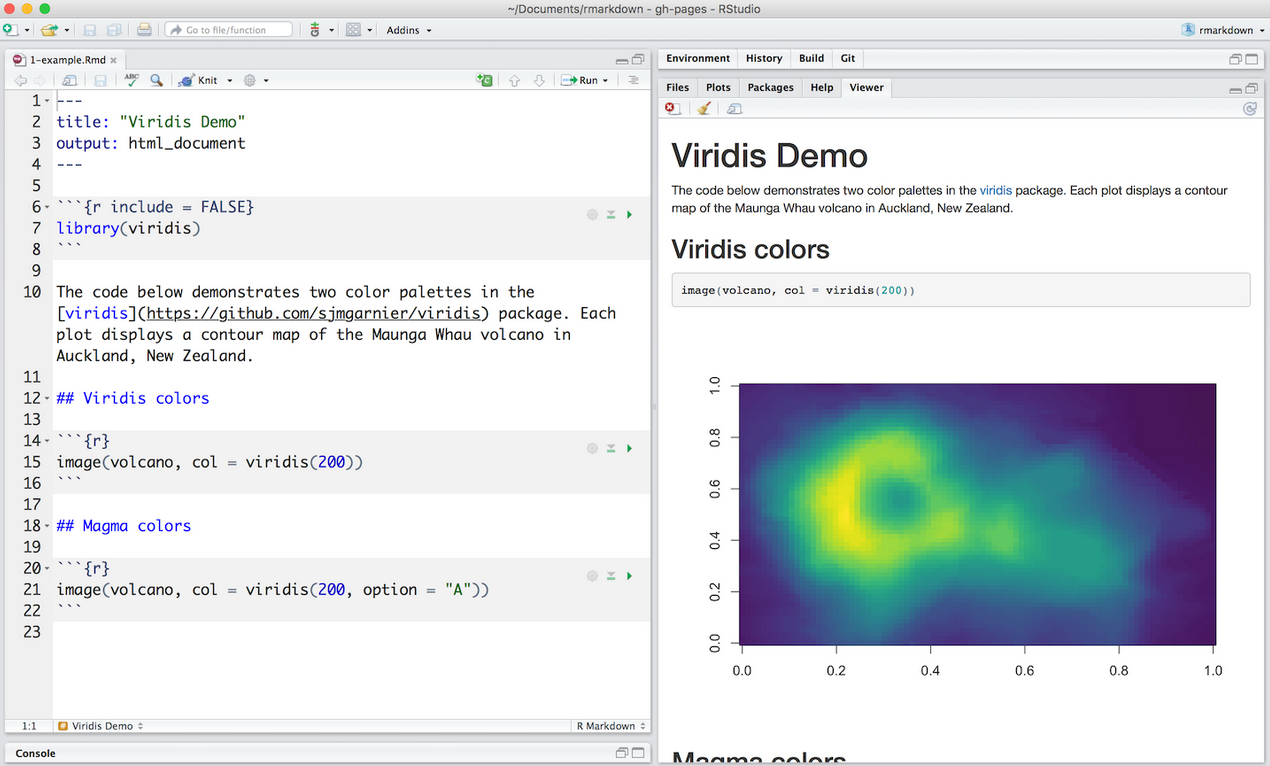
\includegraphics[width=0.75\textwidth,height=\textheight]{fig/rmstudio.png}
\caption{\label{fig:examplermd} Example of an R Markdown file}
\end{figure}

R Markdown provides an authoring framework for data science. You can use a single
R Markdown file to transcript your work, run code, and generate high quality reports, books, websites, articles, theses, blogs, and many more.

In contrast to Quarto (see: \url{https://quarto.org} and \url{https://quarto.org/docs/get-started/hello/rstudio.html}), which is the more recent format, R Markdown is around for some time and hence there are uncountable resources to learn it. For example:

\begin{itemize}
\tightlist
\item
  The \href{https://raw.githubusercontent.com/rstudio/cheatsheets/main/rmarkdown.pdf}{R Markdown Cheatsheet} from posit offers an overview on the most important features of R Markdown.
\end{itemize}

\begin{figure}
\centering
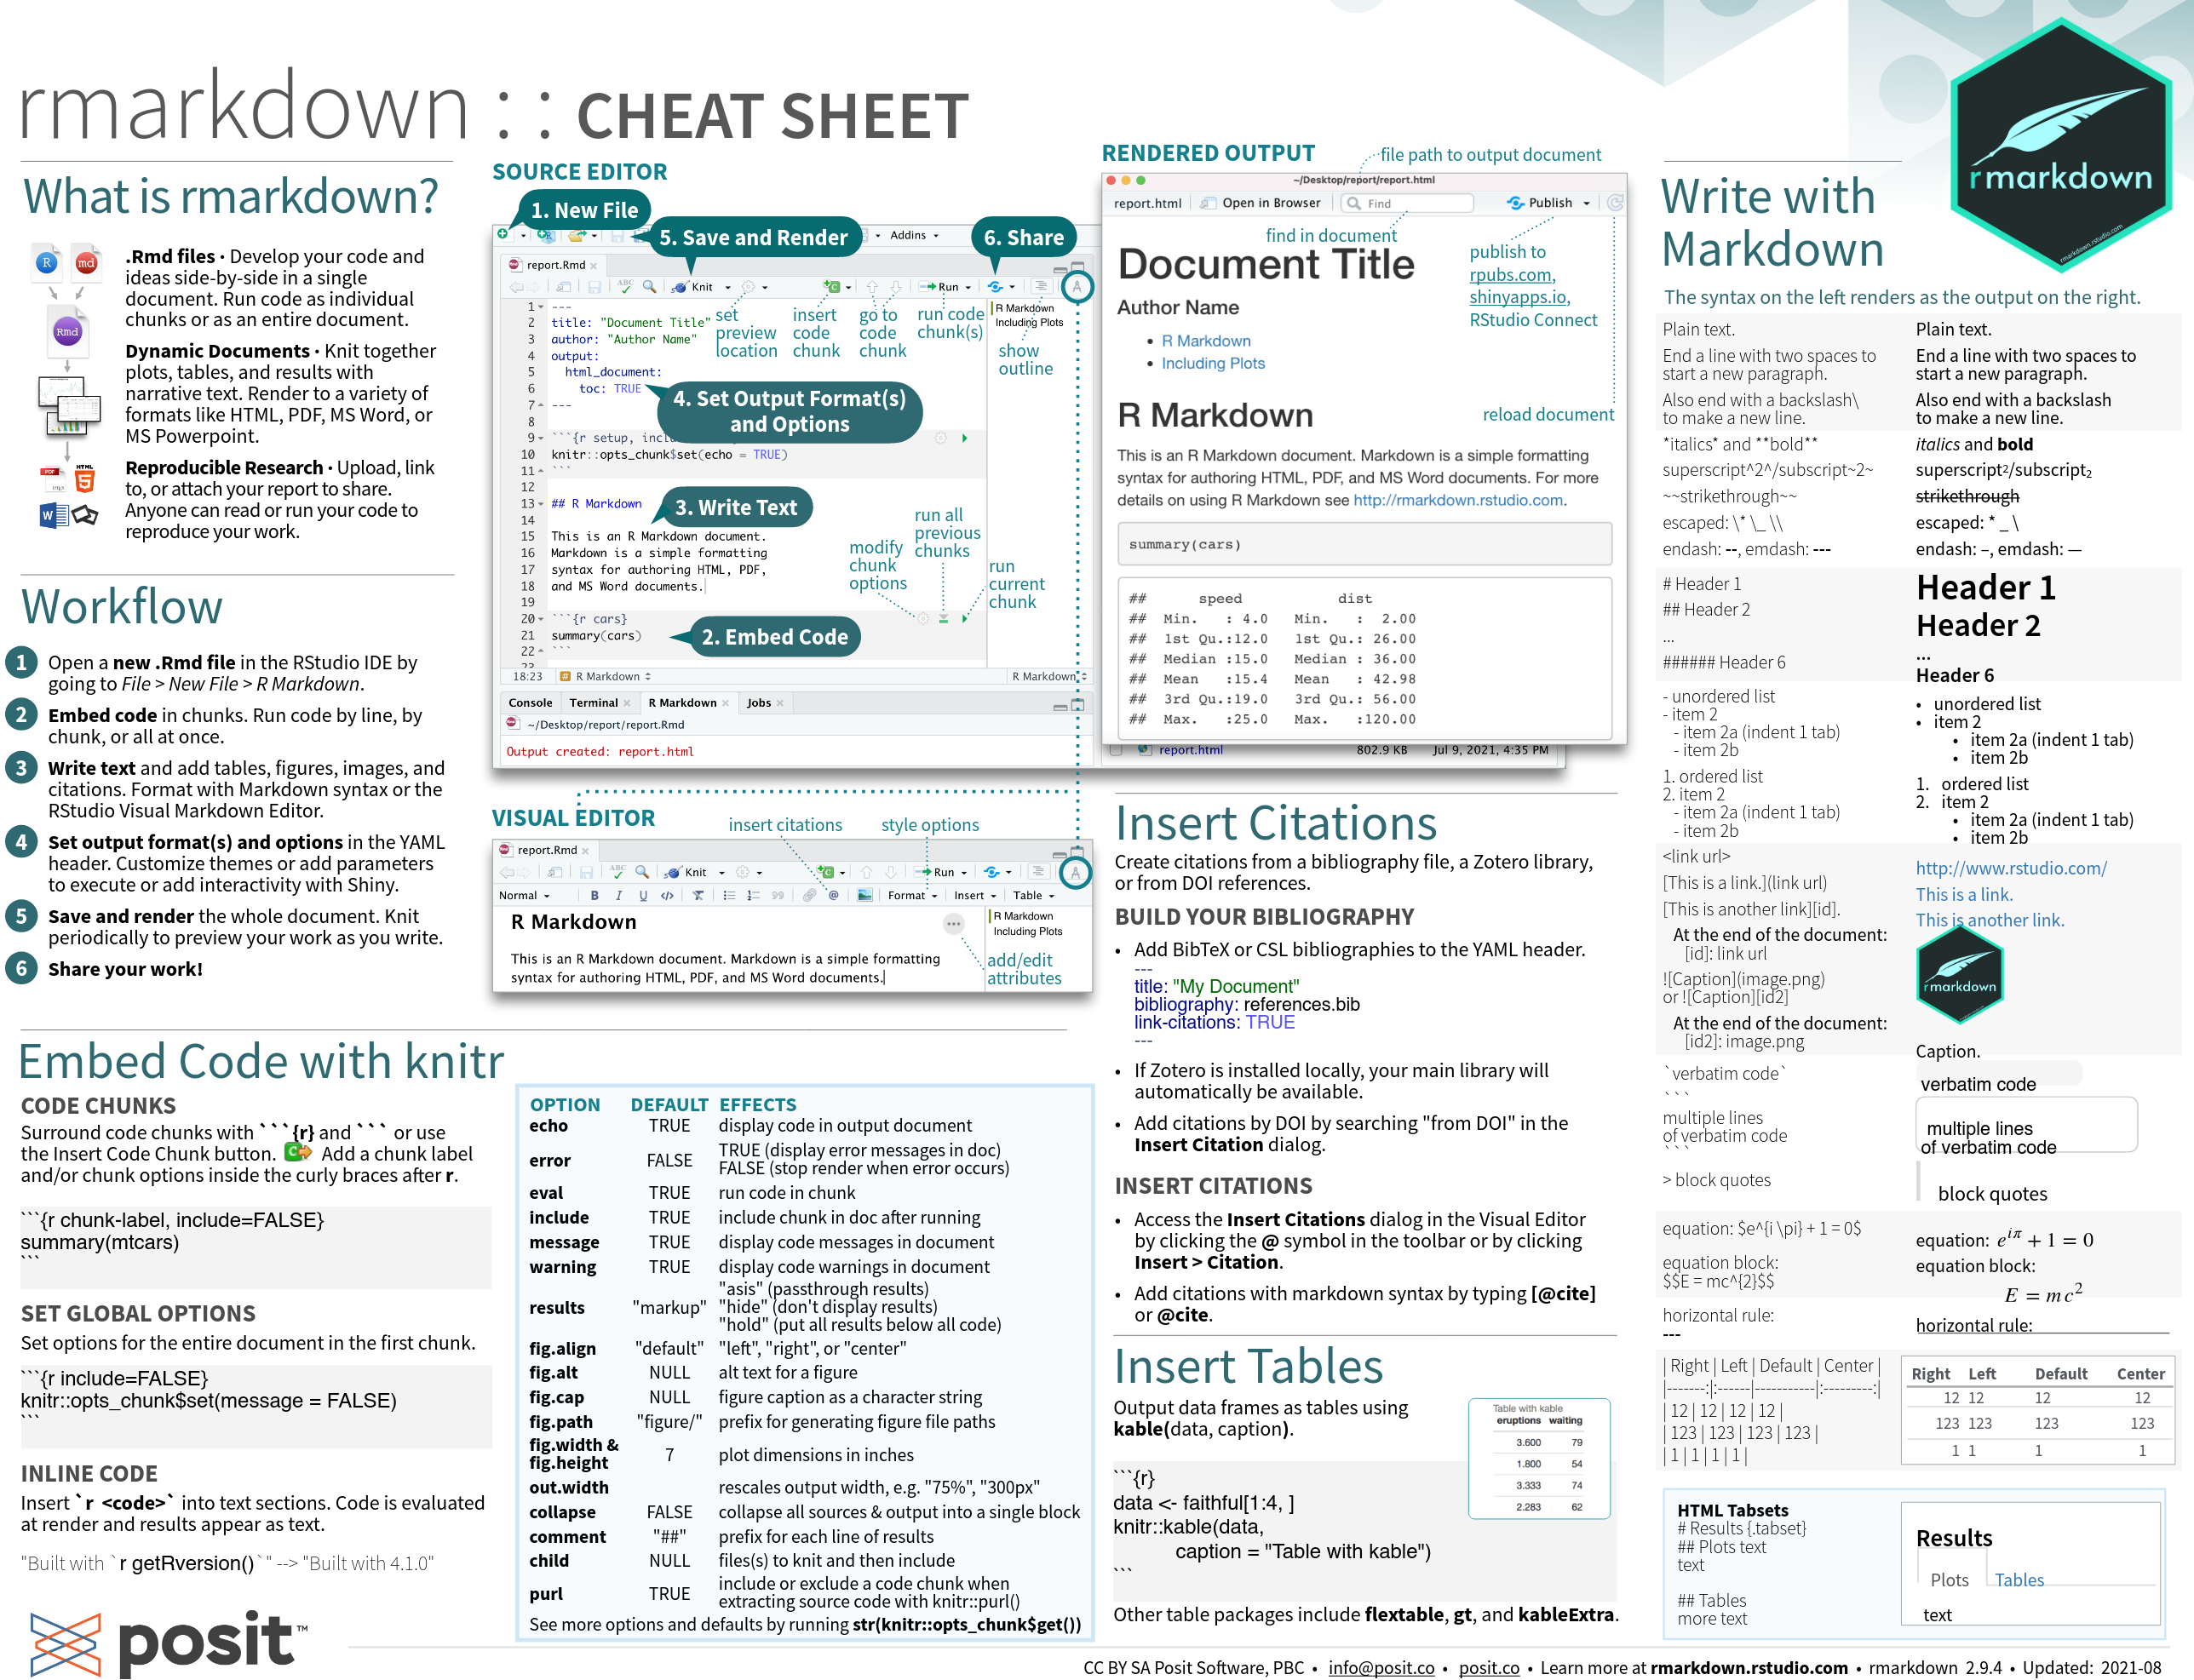
\includegraphics[width=0.5\textwidth,height=\textheight]{fig/rmdcheat.png}
\caption{\label{fig:rmdcheat} R Markdown Cheatsheet from posit}
\end{figure}

\begin{itemize}
\tightlist
\item
  The book \emph{R Markdown Cookbook} by \citet{Xie2020R} offers an introduction. The \href{https://bookdown.org/yihui/rmarkdown-cookbook}{online version of the book} is regularly updated and free of costs.
\end{itemize}


\includegraphics[width=0.25\textwidth,height=\textheight]{fig/rmarkdownbook.png}

\begin{itemize}
\tightlist
\item
  The book \emph{R Markdown: The Definitive Guide} by \citet{Xie2018R} offers a comprehensive introduction. \href{https://bookdown.org/yihui/rmarkdown}{The online version of the book} is regularly updated and free of costs.
\end{itemize}

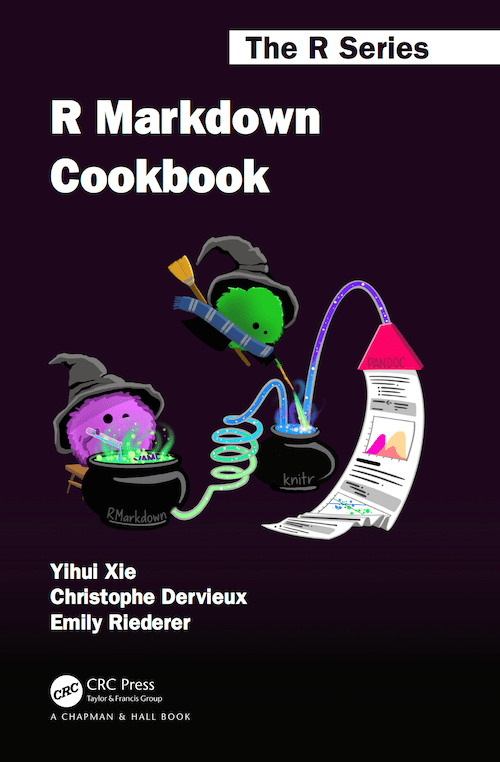
\includegraphics[width=0.25\textwidth,height=\textheight]{fig/rmcb.png}

Please watch the video \href{https://vimeo.com/178485416}{What is R Markdown?} and then study the \href{https://rmarkdown.rstudio.com/lesson-1.html}{R Markdown tutorial from RStudio}.

\begin{exercise}
\protect\hypertarget{exr:rmdfirst}{}\label{exr:rmdfirst}

Start Markdown and R markdown

\begin{enumerate}
\def\labelenumi{\alph{enumi})}
\tightlist
\item
  You can learn Markdown in 10 minutes. Just go to \url{https://www.markdowntutorial.com} and work throught the interactive lessons.
\item
  Now create your first R Markdown file in 3 minutes by doing the following:
\end{enumerate}

\begin{itemize}
\tightlist
\item
  click in RStudio on \emph{File \textgreater{} New File \textgreater{} R Markdown}
\item
  click \emph{OK}
\item
  look for a button entitled \emph{Knit} and click it
\item
  save your file (it will be saved with .Rmd file extension)
\end{itemize}

\begin{enumerate}
\def\labelenumi{\alph{enumi})}
\setcounter{enumi}{2}
\tightlist
\item
  Play around with the file. For example, change the output format can you create a word file or a presentation. Play around with the code chunks. Add a picture that you find somewhere online.
\item
  Set your working directory to the folder where you have saved your first Rmd-file. Can you come up with a way to generate different output format with just one function.
\end{enumerate}

\end{exercise}

\begin{exercise}
\protect\hypertarget{exr:rmdsecond}{}\label{exr:rmdsecond}Please download and open the file ``23-04\_ds-project-desc.Rmd'' from my GitHub account here. Save the file in your working directory and try to run it using the knit function. It may not work properly at first, so you may need to troubleshoot some issues. However, do not worry, as it are usually simply problems that occur and often the error message provided can guide you.

For instance, I use BibTeX to cite literature. It is an excellent method to make the computer perform tedious tasks for you, such as citing papers and generating reference lists based on citation styles. This can save you a significant amount of time and reduce the likelihood of errors while citing literature. The literature I cite is in a separate file, which you can find on one of my GitHub repositories.

Moreover, the YAML header is quite sensitive to spacing and will break you code.
\end{exercise}

\hypertarget{appendix}{%
\chapter{Appendix}\label{appendix}}

\hypertarget{sec:navigation}{%
\section{Navigating the file system}\label{sec:navigation}}

It is essential to know how R interacts with the file system on your computer. Modern operating systems are incredibly user-friendly and try to hide boring and annoying stuff from the customer. In the following, I will try to give a brief introduction on how to navigate around a computer using a DOS or UNIX shell. If you familiar with that, you can skip this part of the notes.

\hypertarget{sec:filesystem}{%
\subsection{The file system}\label{sec:filesystem}}

In this section, I describe the basic idea behind file locations and file paths. Regardless of whether you are using Windows, macOS, or Linux, every file on the computer is assigned a human-readable address, and every address has the same basic structure: it describes a path that starts from a root location, through a series of folders (or directories), and finally ends up at the file.

On a Windows computer, the root is the storage device on which the file is stored, and for many home computers, the name of the storage device that stores all your files is \texttt{C:}. After that comes the folders, and on Windows, the folder names are separated by a backslash symbol \texttt{\textbackslash{}}. So, the complete path to this book on my Windows computer might be something like this:

\begin{verbatim}
C:\Users\huber\Rbook\rcourse-book.pdf
\end{verbatim}

On Linux, Unix, and macOS systems, the addresses look a little different, but they are more or less identical in spirit. Instead of using the backslash, folders are separated using a forward slash, and unlike Windows, they do not treat the storage device as being the root of the file system. So, the path on a Mac might be something like this:

\begin{verbatim}
/Users/huber/Rbook/rcourse-book.pdf
\end{verbatim}

That is what we mean by the \emph{path} to a file. The next concept to grasp is the idea of a working directory and how to change it. For those of you who have used command-line interfaces previously, this should be obvious already. But if not, here is what I mean. The working directory is just whatever folder I am currently looking at. Suppose that I am currently looking for files in Explorer (if you are using Windows) or using Finder (on a Mac). The folder I currently have open is my user directory (i.e., \texttt{C:\textbackslash{}Users\textbackslash{}huber} or \texttt{/Users/huber}). That is my current working directory.

\hypertarget{working-directory}{%
\subsection{Working directory}\label{working-directory}}

The next concept to grasp is the idea of a \emph{working directory} and how to change it. For those of you who have used command line interfaces previously, this should be obvious already. But if not, here's what I mean. The working directory is just ``whatever folder I'm currently looking at''. Suppose that I'm currently looking for files in Explorer (if you're using Windows) or using Finder (on a Mac). The folder I currently have open is my user directory (i.e., \texttt{C:\textbackslash{}Users\textbackslash{}huber} or \texttt{/Users/huber}). That's my current working directory.

The fact that we can imagine that the program is ``in'' a particular directory means that we can talk about moving \emph{from} our current location \emph{to} a new one. What that means is that we might want to specify a new location in relation to our current location. To do so, we need to introduce two new conventions. Regardless of what operating system you're using, we use \texttt{.} to refer to the current working directory, and \texttt{..} to refer to the directory above it. This allows us to specify a path to a new location in relation to our current location, as the following examples illustrate. Let's assume that I'm using my Windows computer, and my working directory is \texttt{C:\textbackslash{}Users\textbackslash{}huber\textbackslash{}Rbook}. The table below shows several addresses in relation to my current one:

\begin{longtable}[]{@{}ll@{}}
\toprule()
Absolute path & Relative path \\
\midrule()
\endhead
\texttt{C:\textbackslash{}Users\textbackslash{}huber} & \texttt{..} \\
\texttt{C:\textbackslash{}Users} & \texttt{..\textbackslash{}..} \\
\texttt{C:\textbackslash{}Users\textbackslash{}huber\textbackslash{}Rbook\textbackslash{}source} & \texttt{.\textbackslash{}source} \\
\texttt{C:\textbackslash{}Users\textbackslash{}huber\textbackslash{}nerdstuff} & \texttt{..\textbackslash{}nerdstuff} \\
\bottomrule()
\end{longtable}

It is quite common on computers that have multiple users to define \texttt{\textasciitilde{}} to be the user's \emph{home directory}. The home directory on a Mac for the `\texttt{huber\textquotesingle{}\textquotesingle{}\ user\ is}/Users/huber/\texttt{.\ And\ so,\ not\ surprisingly,\ it\ is\ possible\ to\ define\ other\ directories\ in\ terms\ of\ their\ relationship\ to\ the\ home\ directory.\ For\ example,\ an\ alternative\ way\ to\ describe\ the\ location\ of\ the}rcourse-book.pdf\texttt{file\ on\ a\ Mac\ would\ be\ \ \textasciigrave{}\textasciigrave{}\textasciigrave{}\ \textasciitilde{}\textbackslash{}Rbook\textbackslash{}rcourse-book.pdf\ \textasciigrave{}\textasciigrave{}\textasciigrave{}\ You\ can\ find\ out\ your\ home\ directory\ with\ the}path.expand()` function:

\begin{Shaded}
\begin{Highlighting}[]
\FunctionTok{path.expand}\NormalTok{(}\StringTok{"\textasciitilde{}"}\NormalTok{)}
\end{Highlighting}
\end{Shaded}

\begin{verbatim}
## [1] "/home/sthu"
\end{verbatim}

Thus, on my machine \textasciitilde{} is an abbreviation for the path /home/sthu.

\begin{Shaded}
\begin{Highlighting}[]
\FunctionTok{getwd}\NormalTok{()}
\end{Highlighting}
\end{Shaded}

\begin{verbatim}
## [1] "/home/sthu/Dropbox/hsf/23-ss/ds"
\end{verbatim}

\hypertarget{sec:navigationR}{%
\subsection{Navigating the file system using the R console}\label{sec:navigationR}}

When you want to load or save a file in R it's important to know what the working directory is. You can find out by using the \texttt{getwd()} command. For the moment, let's assume that I'm using Mac OS or Linux, since things are different on Windows, see section \ref{sec:winbackslash}.
Let's check the current active working directory:

\begin{Shaded}
\begin{Highlighting}[]
\FunctionTok{getwd}\NormalTok{()}
\end{Highlighting}
\end{Shaded}

\begin{verbatim}
## [1] "/home/sthu/Dropbox/hsf/23-ss/ds"
\end{verbatim}

The function \texttt{setwd()} allows to change the working directory:

\begin{Shaded}
\begin{Highlighting}[]
\FunctionTok{setwd}\NormalTok{(}\StringTok{"/Users/huber/Rbook/data"}\NormalTok{)}
\FunctionTok{setwd}\NormalTok{(}\StringTok{"./Rbook/data"}\NormalTok{)}
\end{Highlighting}
\end{Shaded}

The function \texttt{list.files()} lists all the files in that directory:

\begin{Shaded}
\begin{Highlighting}[]
\FunctionTok{list.files}\NormalTok{()}
\end{Highlighting}
\end{Shaded}

\hypertarget{sec:winbackslash}{%
\subsection{Why do the Windows paths use the back-slash?}\label{sec:winbackslash}}

Let's suppose I'm using a computer with Windows. As before, I can find out what my current working directory is like this:

\begin{Shaded}
\begin{Highlighting}[]
\FunctionTok{getwd}\NormalTok{()}
\NormalTok{[}\DecValTok{1}\NormalTok{] }\StringTok{"C:/Users/huber/}
\end{Highlighting}
\end{Shaded}

R is displaying a Windows path using the wrong type of slash, the back-slash. The answer has to do with the fact that R treats the \texttt{\textbackslash{}} character as \emph{special}. If you're deeply wedded to the idea of specifying a path using the Windows style slashes, then what you need to use two back-slashes \texttt{\textbackslash{}\textbackslash{}} whenever you mean \texttt{\textbackslash{}}. In other words, if you want to specify the working directory on a Windows computer, you need to use one of the following commands:

\begin{Shaded}
\begin{Highlighting}[]
\FunctionTok{setwd}\NormalTok{( }\StringTok{"C:/Users/huber"}\NormalTok{ )}
\FunctionTok{setwd}\NormalTok{( }\StringTok{"C:}\SpecialCharTok{\textbackslash{}\textbackslash{}}\StringTok{Users}\SpecialCharTok{\textbackslash{}\textbackslash{}}\StringTok{huber"}\NormalTok{ )}
\end{Highlighting}
\end{Shaded}


  \bibliography{book.bib}

\end{document}
